\documentclass[5p,times]{elsarticle}

\usepackage{amsmath}
\usepackage{array}
\usepackage{booktabs}
\usepackage{graphicx}
\usepackage{url}
\usepackage{xspace}

\newcommand{\plangate}{\textsc{PlanGate}\xspace}
\graphicspath{{figures/}}

\journal{Journal of Systems and Software}

\begin{document}

\begin{frontmatter}

\title{Session-Aware Governance for Multi-Step LLM Service Workflows}

\author[inst1]{Zhuozhen Gao}
\ead{2510268002@mails.szu.edu.cn}

\affiliation[inst1]{
  organization={Shenzhen University},
  city={Shenzhen},
  country={China}
}

\begin{abstract}
Multi-step LLM agents increasingly execute service workflows through tool calls, external APIs, and model-backed backends. Existing gateway and overload-control mechanisms typically govern individual requests, while the useful unit of work is a dependent session whose intermediate steps have no value if the session later fails. This mismatch causes cascade waste, unsafe replay risks, and ambiguous recovery behavior in overloaded agent services. We present \plangate, a session-aware governance gateway for multi-step LLM service workflows. \plangate combines hard admission for invalid or unsafe workflow declarations, adaptive capacity-driven step-0 admission, session commitment for declared plans, continuation-aware ReAct governance, client-cooperative recovery, idempotent side-effect protection, and optional Redis-backed shared state. In the core business-workflow experiment, adaptive governance reduces cascade failures by 31.8 sessions and wasted service time by 544,149 ms relative to disabling capacity admission under high-load failure conditions. End-to-end HTTP+SQLite sanity checks complete 18 runs with zero duplicate side effects and consistent database state. On a six-node CloudLab deployment, Redis-backed shared state recovers 15/15 forced cross-gateway ReAct checkpoints with zero state misses, while memory-local state misses 15/15 cross-gateway resumes. The results show that session-aware governance can reduce workflow waste and improve recovery correctness under constrained or shared backends, while elastic cloud providers define an important boundary for admission-control policies.
\end{abstract}

\begin{keyword}
LLM agents \sep service workflows \sep gateway governance \sep admission control \sep recovery protocol \sep MCP \sep distributed systems
\end{keyword}

\end{frontmatter}

% Elsevier/JSS submissions require highlights as a separate item in the
% submission system. We keep the draft highlights here as comments so that
% they can be copied into the submission metadata without affecting compile.
%
% Highlights:
% - Session-aware governance for multi-step LLM service workflows.
% - Adaptive admission reduces cascade waste under constrained backends.
% - ReAct recovery resumes checkpoints without replaying side effects.
% - HTTP+SQLite and CloudLab checks validate system correctness.
% - Cloud-provider results expose elasticity-driven policy boundaries.

\section{Introduction}
\label{sec:introduction}

Large language model (LLM) agents are moving from single-turn text generation toward multi-step service workflows. A user request may trigger a sequence of tool calls, database updates, external API invocations, and model-backed reasoning steps. These workflows are increasingly exposed through protocols such as the Model Context Protocol (MCP), where agents call tools through gateway-like infrastructure \citep{anthropic2024mcp}. In such settings, the gateway is no longer a passive transport component. It becomes a software control point responsible for admission, overload handling, state continuity, failure recovery, and side-effect safety.

A central difficulty is that conventional service governance operates at the wrong granularity. Rate limits, admission controllers, and overload policies usually decide whether to admit an individual request. Multi-step agent workflows, however, are valuable only at the session level. If an agent completes four tool calls and the fifth is rejected, the earlier calls may become useless. Worse, some earlier calls may already have committed external side effects, such as reservations, payments, ticket updates, or database writes. This creates a mismatch between the \emph{governance unit}, which is often a request, and the \emph{workload unit}, which is a dependent multi-step session.

This mismatch creates three practical failure modes. First, overloaded systems can admit sessions that later fail mid-execution, wasting tool calls, backend latency, model tokens, and service time. We refer to this as cascade waste. Second, recovery can be unsafe if a resumed session replays already completed side-effecting steps. Third, distributed gateway deployments can lose checkpoint state when a session fails on one gateway and resumes through another. These problems are software-system problems rather than model-quality problems: they arise from session state, resource governance, deployment topology, and workflow semantics.

This paper presents \plangate, a session-aware governance gateway for multi-step LLM service workflows. \plangate is implemented as an MCP-compatible reverse proxy between agent clients and tool backends. It separates three governance cases that are often conflated. First, malformed requests, invalid plans, security violations, and unsafe workflow declarations remain hard step-0 rejections. Second, capacity-driven step-0 admission is adaptive: it becomes stricter when backend congestion signals indicate that admitting more sessions would create downstream cascades, and looser when the backend has headroom. Third, continuation requests are governed with session progress in mind, because rejecting a late step wastes more prior work than rejecting a new session.

\plangate also distinguishes the two dominant agent styles. Plan-and-Solve workflows can declare a plan or dependency structure before execution, allowing the gateway to apply budget, dependency, and safety checks at admission time. ReAct workflows reveal future tool calls incrementally, consistent with the interleaved reasoning/action pattern introduced by ReAct \citep{yao2023react}, so the gateway cannot reserve an exact full plan upfront. For these sessions, \plangate uses continuation-aware governance and client-cooperative recovery: after a recoverable failure, the gateway restores checkpoint state and returns a resume payload, while the client continues the remaining workflow without replaying completed side-effecting steps. In distributed deployments, Redis-backed shared state allows checkpoint and reservation state to survive cross-gateway routing.

The paper is organized around five research questions. RQ1 asks whether session-aware governance reduces cascade waste in multi-step service workflows. RQ2 asks whether adaptive step-0 admission avoids the over-rejection of strict admission while still preventing overload-induced cascades. RQ3 asks whether ReAct recovery can resume from checkpoints without replaying completed side effects. RQ4 asks whether the system is deployable with bounded operator overhead and stable configuration behavior. RQ5 asks whether the design remains valid under real service backends and distributed gateway deployment.

Our evaluation is layered rather than based on a single benchmark. Controlled service workflows provide the main cascade and waste result. Mock and vLLM runs isolate backend congestion. Provider smoke tests characterize elasticity. HTTP+SQLite workflows check persisted side effects and idempotency. CloudLab checks distributed shared state. Overhead, ablation, sensitivity, and protocol studies address deployability. The evaluation keeps performance, correctness, deployability, and scope results separate.

Three findings summarize the empirical results. First, under constrained business-workflow load, adaptive governance reduces cascade failures by 31.8 sessions and wasted service time by 544,149 ms relative to disabling capacity admission. Second, ReAct recovery and idempotency checks preserve side-effect safety: the recovery protocol passes 11/11 edge cases, and HTTP+SQLite sanity runs complete with zero duplicate side effects and consistent database state. Third, distributed correctness depends on shared state: in CloudLab, Redis-backed state recovers 15/15 forced cross-gateway ReAct checkpoints with zero state misses, while memory-local state misses 15/15 cross-gateway resumes. At the same time, cloud-provider experiments show that elastic backends can invert admission trade-offs, so \plangate should be interpreted as a constrained/shared-backend governance framework rather than a policy that dominates in every environment.

\subsection{Research Contributions}

This paper makes the following contributions:
\begin{itemize}
  \item \textbf{Problem formulation.} We formulate session-aware governance as a software-systems problem for multi-step LLM service workflows, identifying cascade waste, side-effect replay, and distributed checkpoint loss as core failure modes.
  \item \textbf{System design.} We design \plangate, an MCP-compatible governance gateway that combines hard safety admission, adaptive capacity admission, session commitment for declared plans, continuation-aware ReAct governance, client-cooperative recovery, idempotency, and Redis-backed shared state.
  \item \textbf{Implementation and reproducibility.} We implement \plangate with MCP, HTTP service, SQLite, Redis, vLLM, and cloud-provider adapters, and provide statistical summaries, effect-size tables, scoped findings, and lightweight replay checks.
  \item \textbf{Empirical results.} We evaluate \plangate across controlled workflows, mock and vLLM backends, cloud-provider scope cases, real HTTP+SQLite services, and CloudLab distributed deployment.
\end{itemize}

\subsection{Paper Organization}

The rest of the paper develops this argument as a software-systems study. It first introduces the background and problem statement, then presents the PlanGate architecture and design mechanisms, followed by implementation details, evaluation methodology, experimental results, discussion, threats to validity, related work, and conclusion.

\section{Background and Motivation}
\label{sec:background}

\subsection{Multi-Step LLM Service Workflows}

LLM agents increasingly act as workflow coordinators. Instead of producing a single response, an agent may search for information, call a pricing service, reserve inventory, update a ticket, authorize a payment, and summarize the result. Each step can be implemented as an MCP tool call, an HTTP API call, a database update, or a model-backed computation. From a software-systems perspective, this workload resembles a service workflow: a user-facing task is decomposed into an ordered set of service invocations whose correctness depends on control flow, data dependencies, and side-effect management, echoing long-standing service-oriented computing, workflow-pattern, and saga concerns \citep{papazoglou2003soc,papazoglou2008roadmap,vanderAalst2003workflowpatterns,garciamolina1987sagas}.

These workflows differ from traditional independent RPC workloads in two ways. First, tool invocations within a session are not interchangeable requests. A later call depends on earlier observations, and a rejected later step may invalidate all earlier work. Second, some tools are side-effecting. A workflow may reserve a flight, create an order row, apply a credit, or update a support ticket. Retrying or resuming such workflows requires idempotency and checkpoint semantics, not only request retransmission. These properties make multi-step agent workloads a natural target for service governance rather than a pure model-evaluation problem.

\subsection{Agent Styles and Available Information}

\plangate targets two common agent execution styles. We use Plan-and-Solve to denote a declared-plan workflow mode, not a claim about a specific prompting benchmark. Such workflows expose a plan before execution. The plan may include a step list, dependency graph, budget declaration, or other metadata that allows a gateway to reason about resource needs before the first tool executes. This enables stronger admission semantics: the gateway can reject malformed or unsafe declarations, check budget feasibility, and bind the admitted session to a commitment scope.

ReAct-style workflows expose less information upfront. The agent decides the next tool call after observing the previous result, so the gateway cannot know the full future plan at step 0 \citep{yao2023react}. Treating ReAct as if it had a declared plan would overstate what the infrastructure can guarantee. Instead, ReAct governance must be incremental: the gateway observes session progress, assigns continuation value to already completed work, and provides a recovery point when a recoverable failure occurs. In \plangate, ReAct recovery is client-cooperative: the gateway restores checkpoint state and returns a resume payload, while the client remains responsible for issuing the remaining tool calls.

\subsection{Why Request-Level Governance Is Insufficient}

Most existing gateway policies make decisions per request. This is appropriate for stateless RPC traffic, but it is incomplete for dependent sessions. A request-level limiter can reject a tool call at step 5 even if steps 1--4 have already consumed backend capacity. A delay-sensitive price controller can increase prices mid-session because the system became congested after the session started. A local checkpoint store can recover a session only if the resume request reaches the same gateway process. These decisions may be locally reasonable while globally wasteful at the session level.

The mismatch produces a characteristic failure pattern: a session is admitted, consumes partial work, and then fails before completion. The failure is worse than a step-0 rejection because the system has already consumed service time, tokens, and possibly durable side effects. The goal of session-aware governance is not to eliminate rejection. Rejection is necessary under overload and for invalid workflows. The goal is to move unavoidable capacity rejection earlier, preserve admitted progress when possible, and prevent unsafe replay during recovery.

\subsection{Motivating Service-Engineering Requirements}

The service-engineering requirements for such workloads are broader than throughput and latency. A useful gateway must preserve workflow semantics, expose a clear recovery contract, keep side effects idempotent, and remain deployable in multi-gateway systems. This motivates four requirements:

\begin{itemize}
  \item \textbf{R1: Session-level admission and continuation.} Admission should distinguish new sessions from continuation steps and should account for the increasing waste of late-session rejection.
  \item \textbf{R2: Explicit recovery contract.} Recovery should restore progress without replaying completed side-effecting steps or automatically executing future tools without client intent.
  \item \textbf{R3: Idempotent side-effect integrity.} Service workflows must use idempotency and final-state checks so that retries and resumes do not duplicate durable operations.
  \item \textbf{R4: Distributed checkpoint availability.} In multi-gateway deployments, reservations and checkpoints must be available across gateway boundaries, or cross-node resume will lose state.
\end{itemize}

These requirements motivate an evaluation hierarchy that separates controlled waste-reduction experiments from side-effect, backend-realism, and distributed-state evidence.

\section{Problem Statement and Research Questions}
\label{sec:problem}

\subsection{System Model}

We consider a service workflow initiated by an LLM agent client. A workflow session consists of a sequence of tool invocations $s = (r_1, r_2, \ldots, r_k)$ routed through a gateway to one or more backend services. Each request may consume service time, model tokens, queue capacity, and possibly durable side effects. A session succeeds only if the workflow reaches a valid terminal state. A session can be rejected at step 0 before any tool execution, or it can fail after admission because a later step is rejected, times out, or encounters a recoverable interruption.

We distinguish three classes of rejection. \emph{Hard rejection} applies to malformed requests, invalid workflow declarations, security violations, unsafe plan amendments, or inconsistent recovery tokens. These failures should remain strict because admitting them would violate system invariants. \emph{Capacity rejection} applies when backend load suggests that admitting more work would cause queue buildup or downstream cascade. This rejection should be adaptive because the appropriate policy depends on actual congestion. \emph{Continuation rejection} applies to already admitted sessions; it is expensive because it can waste prior work and should therefore be governed differently from new-session admission.

\subsection{Failure Metrics}

The primary failure mode is cascade waste. A cascade failure occurs when an admitted session fails after completing at least one step. The wasted work includes completed tool calls, service time, model tokens, and side-effect management overhead that no longer contribute to a successful workflow. We also track step-0 rejection, because moving rejection earlier can reduce waste but may reduce availability. These metrics create a trade-off: a policy that admits everything can maximize raw success under elastic backends but may create large cascade waste under hard capacity; a policy that rejects too aggressively can reduce waste while denying workflows that could have completed.

For recovery, we track whether the gateway returns a valid resume payload, whether the client can continue after resume, whether completed steps are replayed, and whether durable side effects remain unique. For distributed deployments, we track cross-gateway resume, state misses, duplicate admissions, and final database consistency. These metrics reflect service correctness rather than model accuracy. Table~\ref{tab:core_metrics} summarizes the core terms used throughout the evaluation.

\begin{table}[t]
\centering
\caption{Core service-governance metrics used in the paper.}
\label{tab:core_metrics}
\footnotesize
\begin{tabular}{@{}>{\raggedright\arraybackslash}p{0.30\columnwidth}>{\raggedright\arraybackslash}p{0.60\columnwidth}@{}}
\toprule
\textbf{Metric} & \textbf{Meaning} \\
\midrule
Cascade failure & An admitted session fails after at least one completed step. \\
Wasted service time & Service time consumed by sessions that do not reach a valid terminal state. \\
Step-0 rejection & Rejection before workflow work begins. \\
Duplicate side effect & Repeated durable operation under the same logical workflow. \\
State miss & A resume path cannot find checkpoint or reservation state. \\
\bottomrule
\end{tabular}
\end{table}

\subsection{Research Questions}

The paper is organized around five research questions:

\begin{description}
  \item[\textbf{RQ1.}] Does session-aware governance reduce cascade failures and wasted service work in multi-step service workflows under constrained backend capacity?
  \item[\textbf{RQ2.}] How does adaptive capacity-driven step-0 admission trade off early rejection against mid-session cascade compared with always-strict and no-capacity-step0 policies?
  \item[\textbf{RQ3.}] Can client-cooperative ReAct recovery resume from checkpoints, continue remaining workflow steps, and avoid replaying completed side-effecting operations?
  \item[\textbf{RQ4.}] Does the gateway introduce bounded operator overhead, and do its qualitative signals persist under configuration and component variations?
  \item[\textbf{RQ5.}] Does the design hold across external settings: HTTP+SQLite services, model-backed backends, cloud providers, and CloudLab?
\end{description}

The research questions separate effectiveness, correctness, deployability, and scope. For example, the HTTP+SQLite and CloudLab studies are not used to argue raw performance superiority; they check side-effect safety and distributed correctness. Conversely, the controlled business-workflow experiments provide the main basis for cascade-waste reduction.

\subsection{Scope and Non-Goals}

\plangate is not a model-quality benchmark and does not attempt to improve the reasoning accuracy of an LLM agent. It governs service workflow execution after the agent chooses tools. The system also does not claim production Redis high availability, Byzantine security against malicious clients, or fully automatic server-side recovery. Recovery is client-cooperative by design: the gateway exposes a safe resume point, and the client continues the remaining workflow. Finally, the paper does not claim that one admission policy dominates in all environments. Cloud-provider experiments show that elastic providers can hide backend congestion and change the best raw-success trade-off.

\section{PlanGate Overview}
\label{sec:overview}

\subsection{Architecture}

\plangate is a gateway layer between agent clients and backend tools. The client sends MCP-compatible tool calls with session metadata. The gateway classifies each request, applies admission and recovery logic, and forwards admitted calls to the backend. The backend may be a mock service, a vLLM-backed tool service \citep{kwon2023vllm}, a cloud-provider-backed tool service, or an HTTP business service backed by SQLite. In distributed deployments, multiple gateway processes share reservation and checkpoint state through Redis. Figure~\ref{fig:plangate_architecture_lifecycle} shows the architecture and workflow lifecycle.

The architecture has six logical components. The admission controller handles hard workflow rejection and adaptive capacity admission. The session manager tracks active sessions, commitments, and continuation state. The ReAct checkpoint manager records completed progress for recoverable sessions. The recovery protocol returns explicit resume payloads and requires client-side continuation. The idempotency layer protects side-effecting tools from duplicate writes. The shared-state adapter stores reservations and checkpoints either in process-local memory or in Redis.

\begin{figure*}[t]
\centering
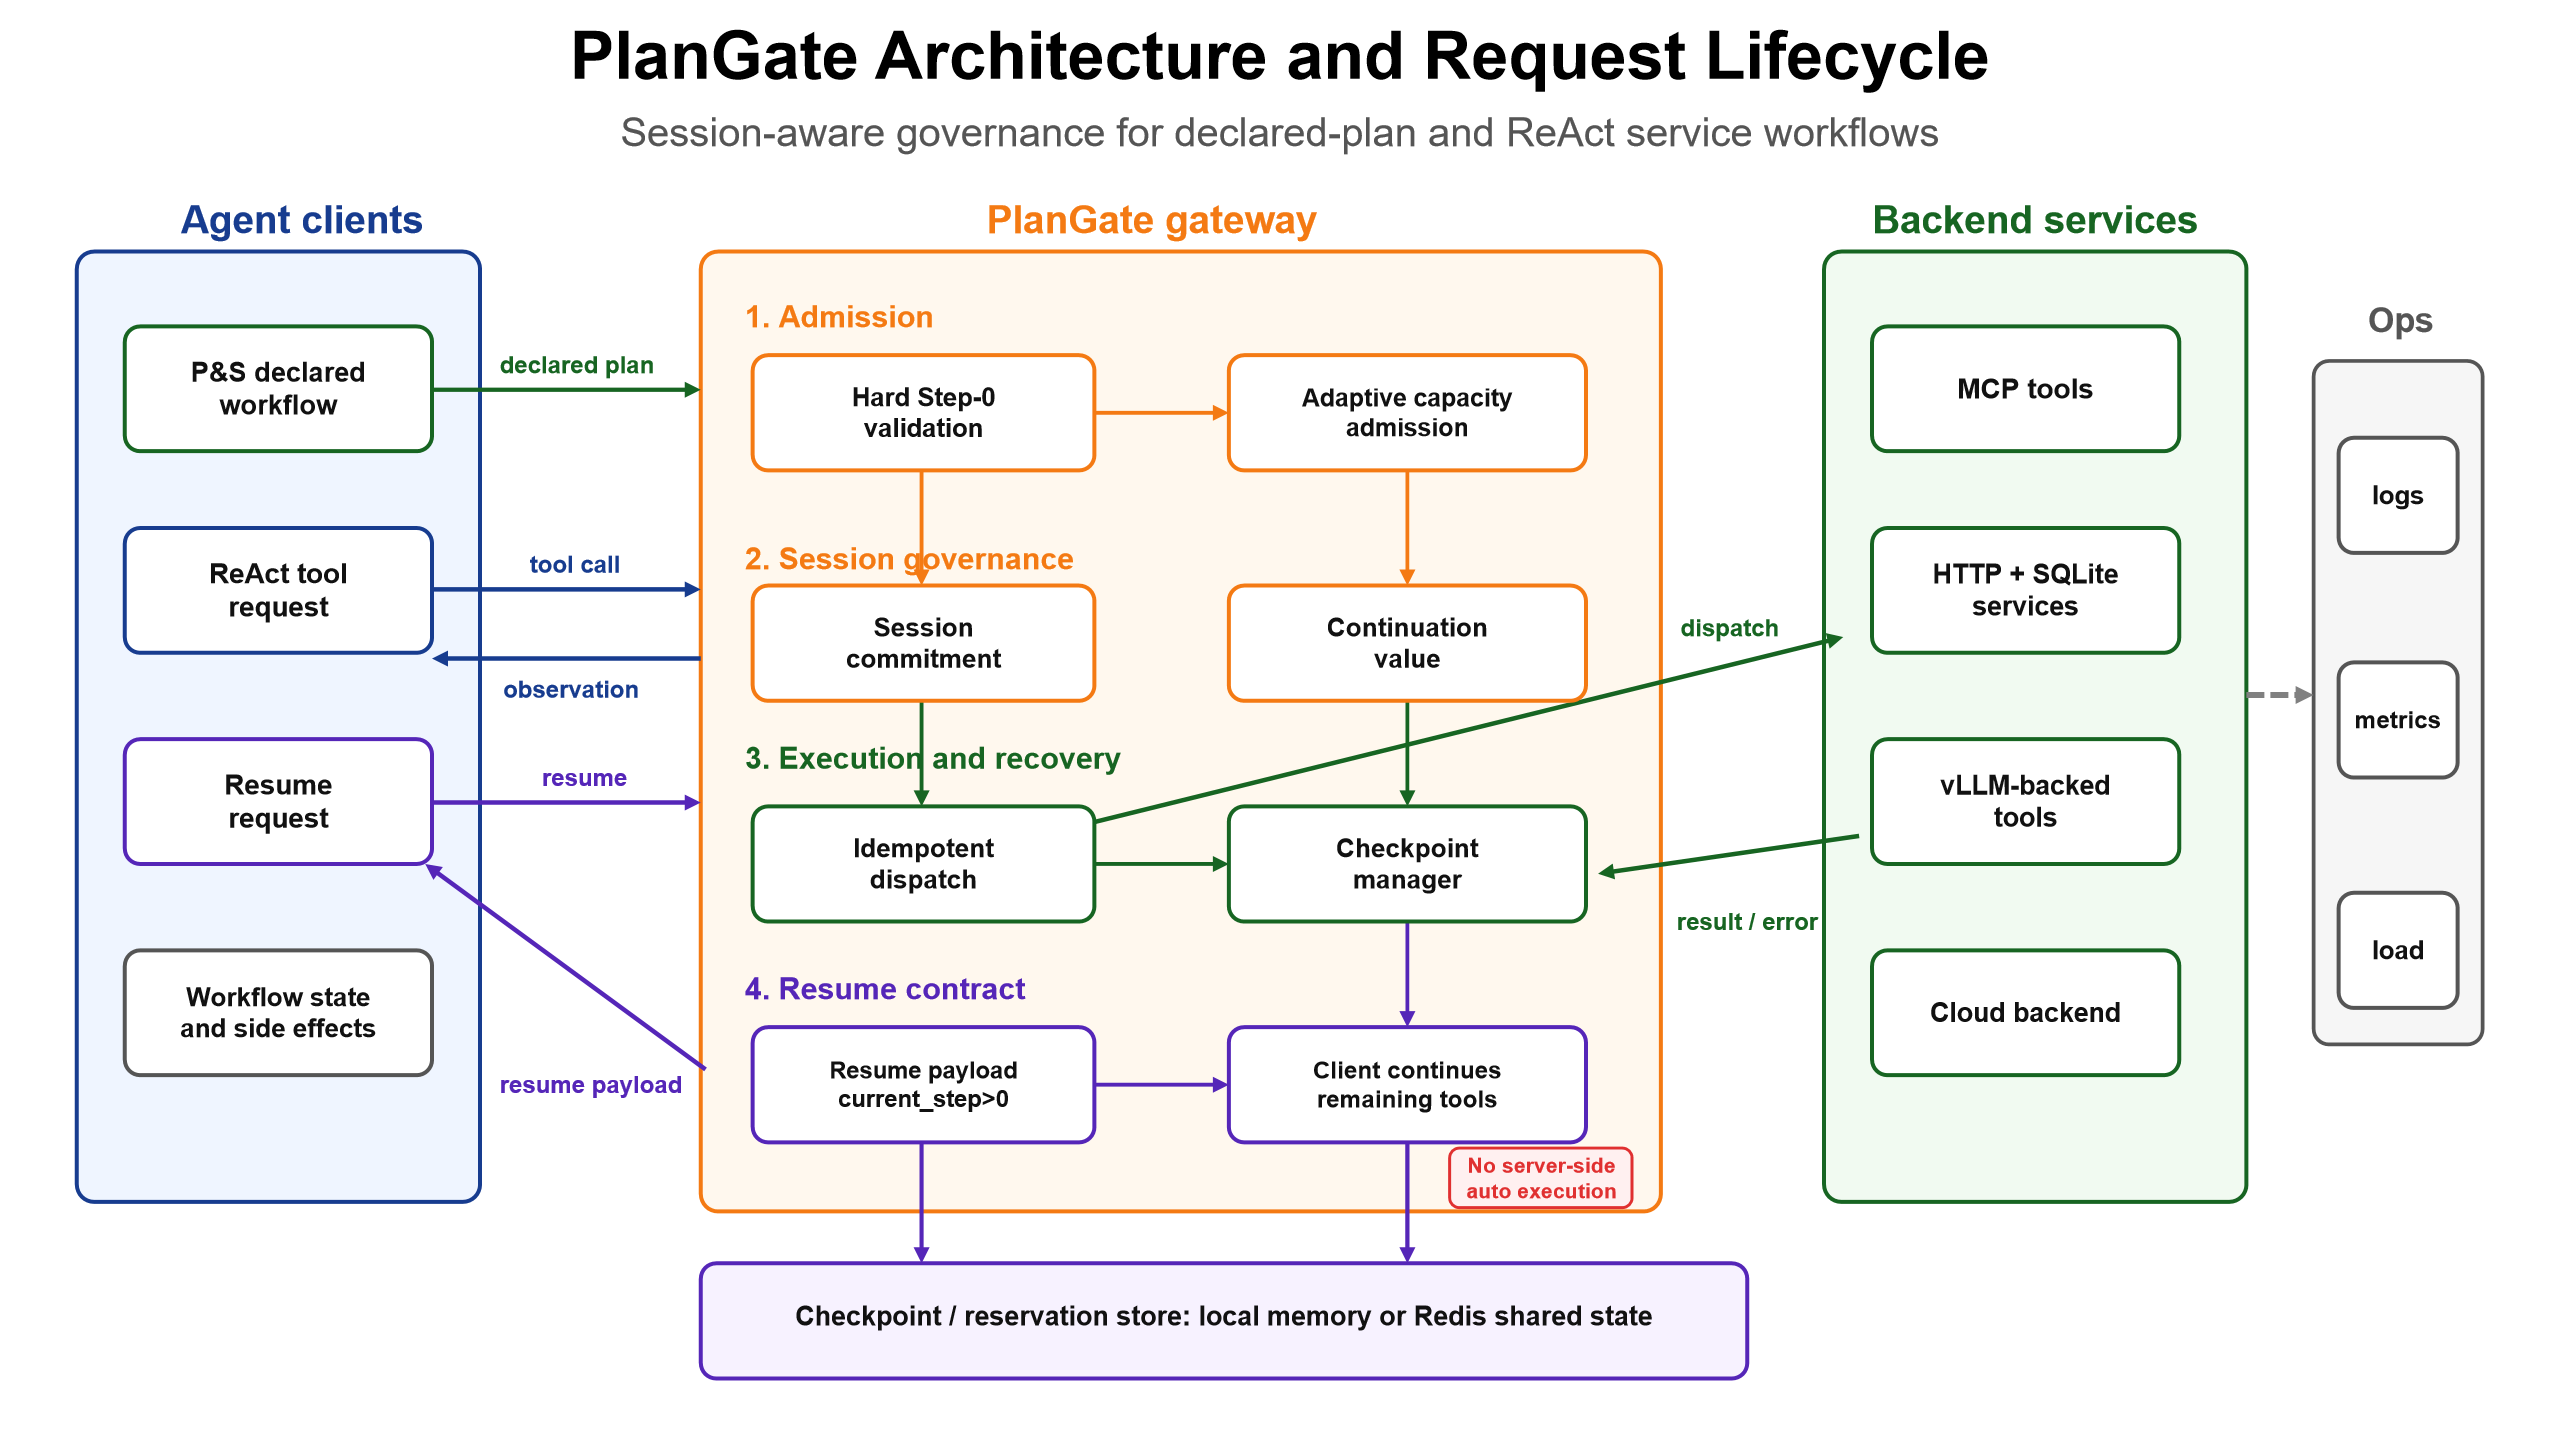
\includegraphics[width=0.88\textwidth]{fig_plangate_architecture_lifecycle_reference.png}
\caption{PlanGate architecture and workflow lifecycle. The gateway sits between agent clients and tool backends, separating hard validation, adaptive capacity admission, session tracking, recovery, idempotency, and shared-state lookup.}
\label{fig:plangate_architecture_lifecycle}
\end{figure*}

\begin{table*}[t]
\centering
\caption{PlanGate component responsibilities and design boundaries.}
\label{tab:overview_components}
\footnotesize
\begin{tabular}{@{}>{\raggedright\arraybackslash}p{0.20\textwidth}>{\raggedright\arraybackslash}p{0.49\textwidth}>{\raggedright\arraybackslash}p{0.24\textwidth}@{}}
\toprule
\textbf{Component} & \textbf{Responsibility} & \textbf{Boundary} \\
\midrule
Adaptive admission & Separates hard rejection from capacity-driven admission and controls the early-reject versus cascade trade-off. & Does not guarantee raw-success dominance. \\
Session commitment & Uses declared workflow information for stronger admission and continuation semantics. & Applies within declared scope and valid metadata. \\
ReAct checkpointing & Preserves completed ReAct progress after recoverable interruption. & Does not auto-execute future tools. \\
Recovery protocol & Exposes a resume point and requires explicit client continuation. & Not transparent server-side replay. \\
Idempotency layer & Prevents duplicate durable side effects during retry and resume. & Tested workflow-side idempotency, not complete malicious-client security. \\
Shared-state adapter & Shares reservations and checkpoints across gateway processes. & Not production Redis HA or fault tolerance. \\
\bottomrule
\end{tabular}
\end{table*}

\subsection{Request Lifecycle}

At the start of a workflow, the gateway first applies hard validation. Invalid plans, malformed metadata, unsafe amendments, and inconsistent recovery tokens are rejected before backend execution. If the request is a new session and the only concern is backend capacity, \plangate applies adaptive step-0 admission. The policy is intentionally not always strict: strict admission can over-reject when the backend has headroom or when a cloud provider absorbs load, while disabling capacity admission can create large cascade waste under constrained backends.

For a declared workflow, \plangate records a session commitment and tracks the admitted scope. For a ReAct workflow, the gateway records progress as the client issues tools. When a recoverable failure occurs, the checkpoint manager marks the session recoverable and records the last completed safe point. A resume request with the same session identity returns a payload indicating that the session was recovered, the current step is greater than zero, and client continuation is required. The gateway does not execute future tools by itself.

For side-effecting services, the tool layer attaches idempotency keys and checks database consistency. This is essential because recovery without idempotency can duplicate external operations. The evaluation later checks this path with HTTP business services backed by SQLite, but the overview only defines the control path.

\subsection{Deployment Modes}

\plangate supports single-gateway and multi-gateway deployment. In a single-gateway setting, in-memory state is sufficient for local experiments and small deployments. In a multi-gateway setting, request routing may send a failure and its resume request to different gateway processes. Memory-local state cannot reliably recover such sessions because the checkpoint may exist only in the gateway that handled the failure. Redis-backed shared state addresses this by externalizing reservation and checkpoint lookup.

\subsection{Design Boundary}

Table~\ref{tab:overview_components} summarizes component responsibilities and limits. The evaluation later maps these components to concrete studies. The key point is that \plangate's contribution is not ``always reject earlier'' or ``always admit more.'' Its contribution is a session-aware control plane that makes admission, continuation, recovery, and shared-state decisions explicit and measurable. Under constrained or shared backends this can reduce cascade waste; under elastic cloud-provider backends the best raw-success policy can differ, so deployment context matters.

\section{Design}
\label{sec:design}

\subsection{Design Principles}

\plangate follows three design principles. First, workflow validity and capacity pressure are separated. Malformed metadata, invalid plans, unsafe amendments, and inconsistent recovery tokens remain hard failures that are rejected before backend execution. Capacity pressure is governed separately because its correct handling depends on recent load, queueing behavior, and provider elasticity.

Second, session progress changes admission cost. Rejecting a new session before work begins wastes little service work; rejecting a continuation step after several completed tools can waste service time, tokens, and side-effect management. \plangate therefore treats new-session admission and continuation admission differently, without assuming that every continuation must be admitted.

Third, recovery is explicit and idempotent. The gateway exposes a resume point but does not replay completed side-effecting operations or execute future tools on behalf of the client. The client-cooperative contract keeps recovery observable, while idempotency keys protect durable operations from duplicate writes.

\subsection{Admission and Commitment}

For declared-plan workflows, \plangate uses admission as a commitment point. A client may provide a session identifier, declared steps, dependencies, budget information, or amendment intent. The gateway validates this metadata before backend execution and rejects requests that violate the declared workflow contract. When the workflow is admitted, the session manager records an active commitment and checks later continuation steps against that scope. This mechanism applies to workflows that expose enough structure for upfront reasoning; it is not treated as a full-plan guarantee for ReAct sessions.

\subsection{Adaptive Capacity Admission}

The adaptive module only applies to capacity-driven decisions; hard validation is handled before this path. The module tracks recent cascade behavior, recoverable-error signals, active sessions, and backend pressure, and combines them into a governance-intensity setting. This setting determines how aggressively new sessions should be rejected before execution.

The design is evaluated through three admission policies. A \emph{strict} policy rejects early under capacity pressure. A \emph{no-capacity-step0} policy disables capacity-driven step-0 rejection. The \emph{adaptive} policy keeps hard rejection but changes capacity admission according to observed pressure. This comparison is necessary because constrained local backends and elastic cloud providers can prefer different raw-success trade-offs.

\subsection{ReAct Checkpointing and Recovery}

ReAct workflows choose tools incrementally, so \plangate cannot reserve a complete future plan. Instead, each tool call carries session and step metadata. The gateway records completed progress after successful tool execution and uses this state to distinguish new work from continuation work.

When a recoverable failure occurs, \plangate marks the session as checkpointed. A resume request with the same session identity and explicit recovery mode restores the checkpoint and returns a payload describing the recovered state, current step, and requirement for client continuation. The gateway does not execute future tools during recovery. This boundary prevents hidden server-side replay and keeps future tool choice under client control. Figure~\ref{fig:react_recovery_protocol} summarizes this client-cooperative protocol.

\begin{figure*}[t]
\centering
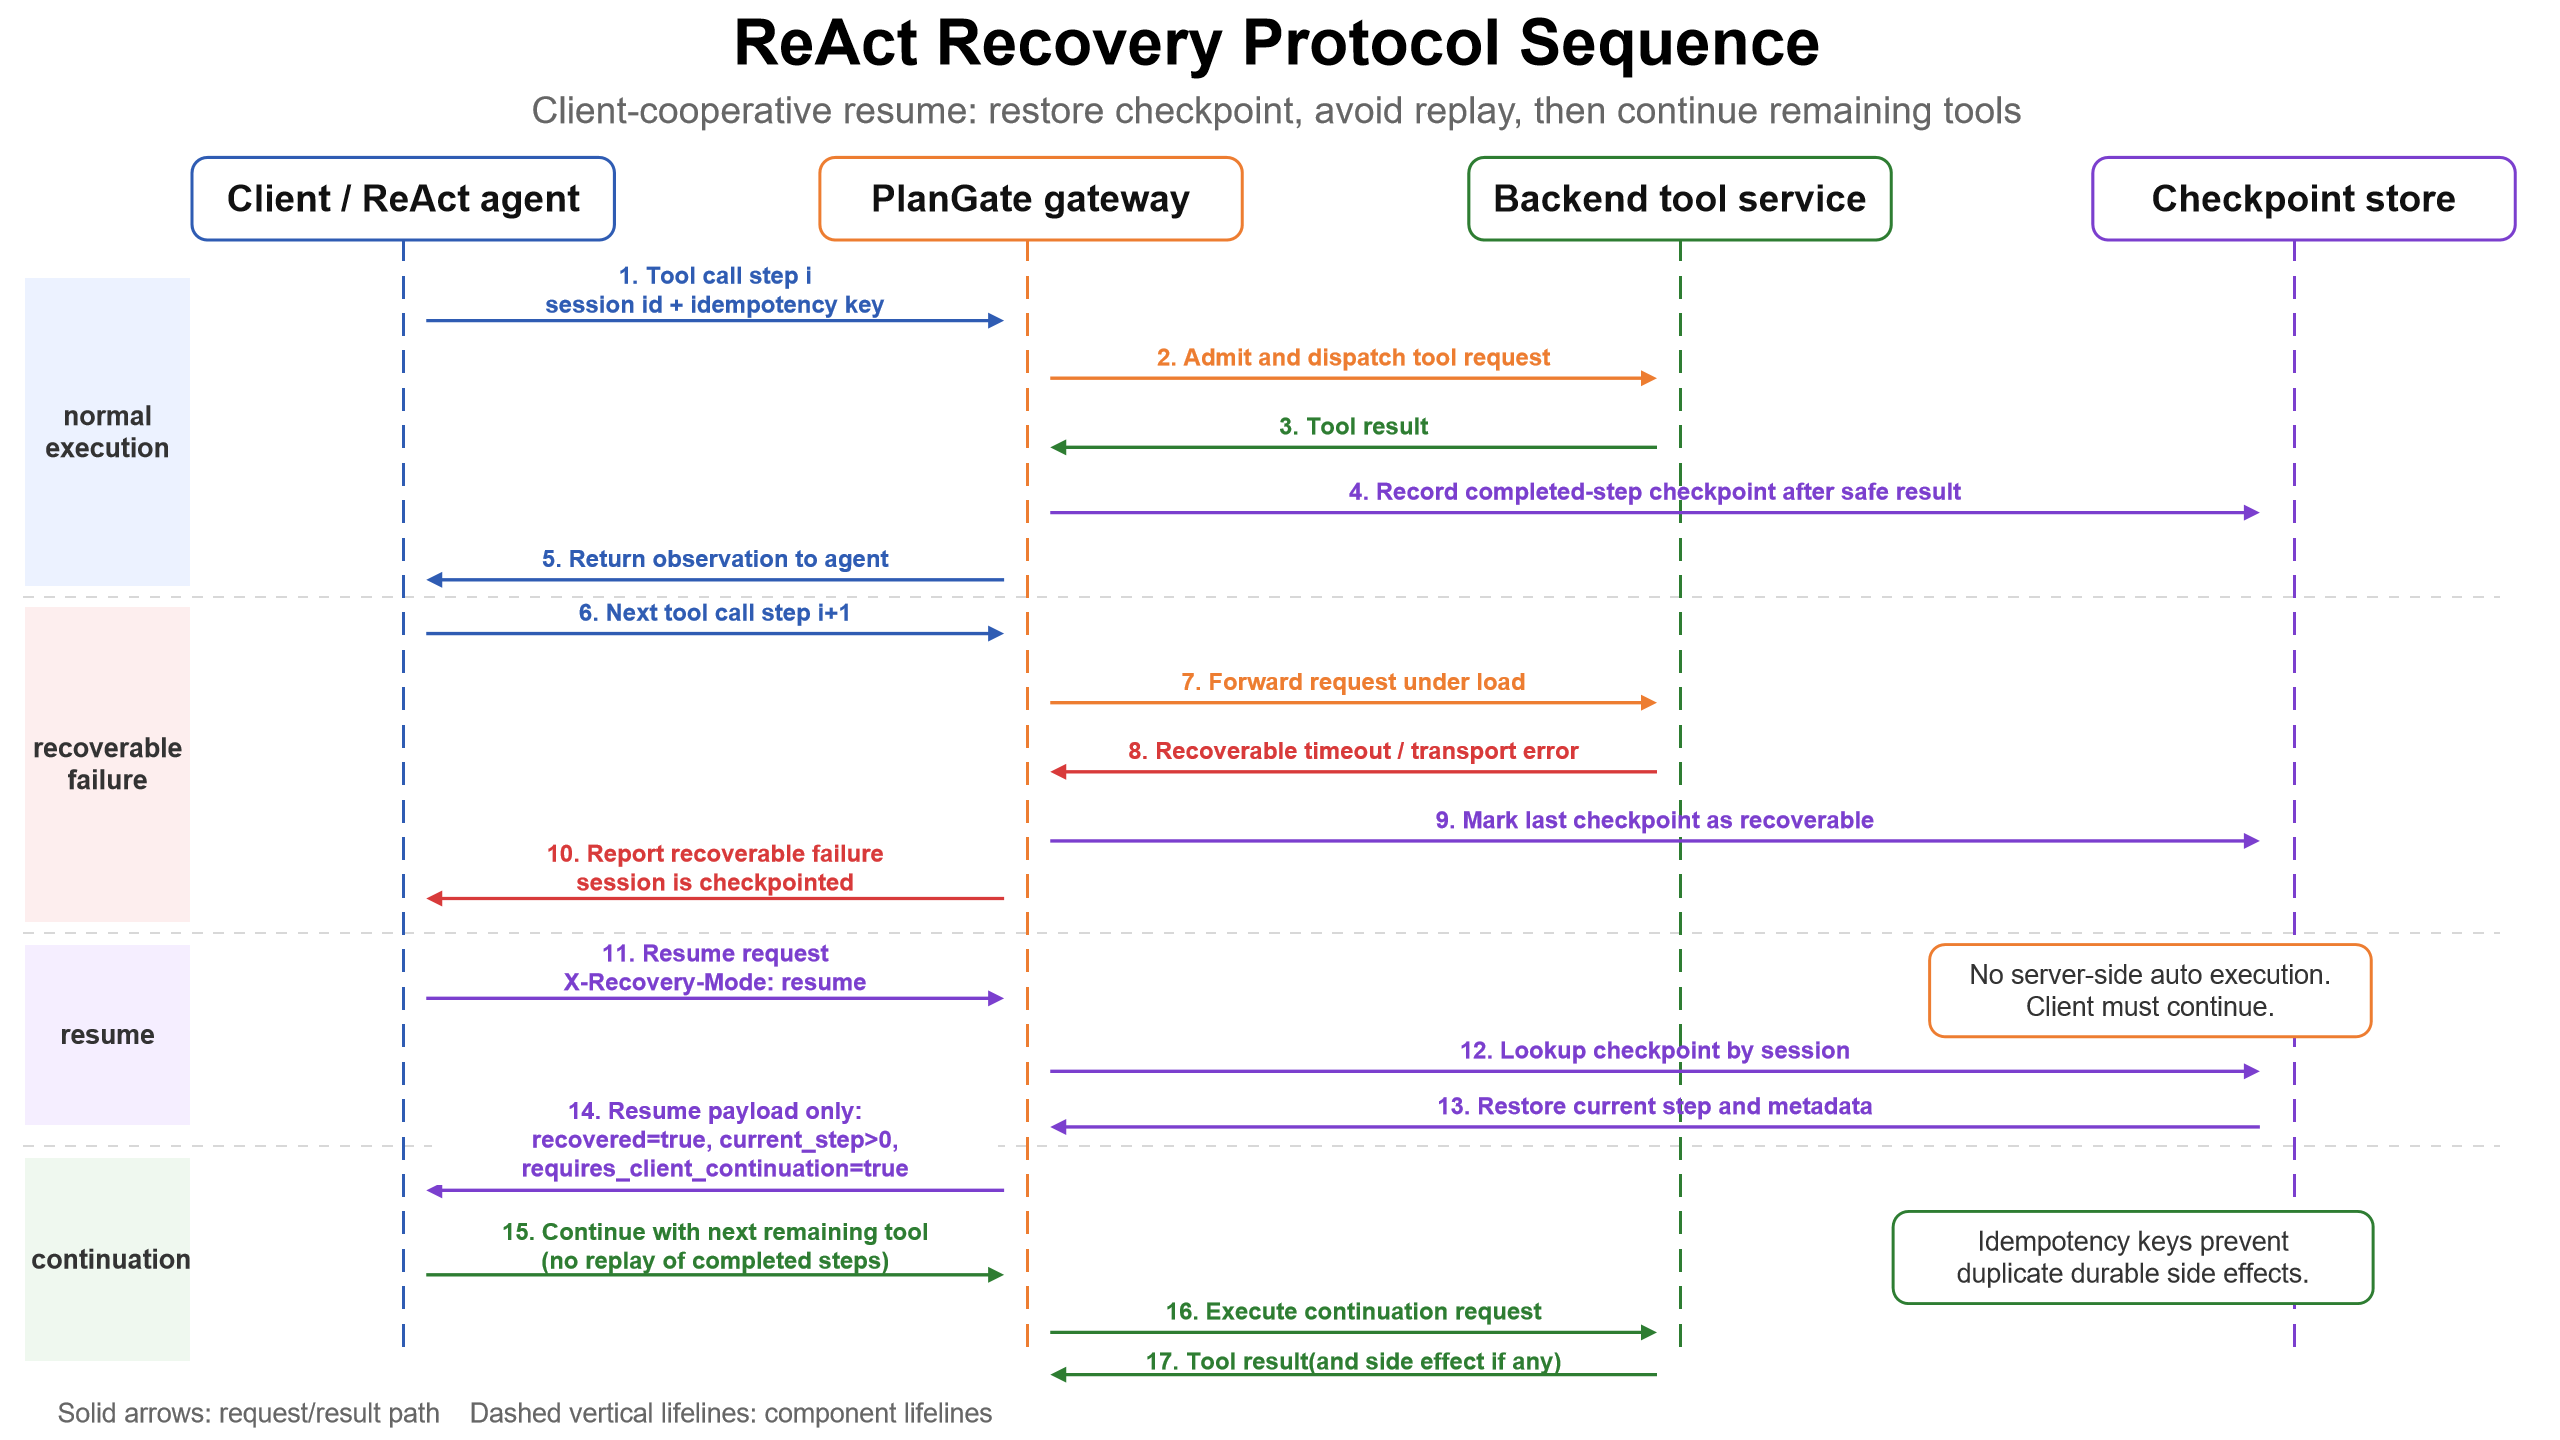
\includegraphics[width=0.88\textwidth]{fig_react_recovery_protocol_sequence.png}
\caption{Client-cooperative ReAct recovery protocol. The gateway restores checkpointed progress and returns a resume payload; the client then continues the remaining workflow steps explicitly.}
\label{fig:react_recovery_protocol}
\end{figure*}

\subsection{Side-Effect Integrity}

Service workflows often contain durable operations. The mechanism assumes that side-effecting tools expose stable idempotency keys and side-effect identifiers. Normal retry should return the same logical operation result rather than create a duplicate write; recovery should not replay completed side-effecting steps. The evaluation uses HTTP services backed by SQLite to check this property, but the design itself only requires idempotency keys, checkpointed progress, and final-state validation.

\subsection{Distributed Shared State}

In a single gateway, session state can be kept in memory. In a multi-gateway deployment, a failure and its resume request may reach different gateway processes, so process-local checkpoints are insufficient. \plangate therefore supports a shared-state adapter for reservations, checkpoints, and recovery metadata. Redis is used as a shared lookup service in the current implementation, while memory-local state remains a diagnostic control. This design supports cross-gateway recovery but does not claim production Redis high availability, node-crash recovery, or fault-tolerant store management.

\section{Implementation}
\label{sec:implementation}

\plangate is implemented in Go as an MCP-compatible gateway. It exposes HTTP handlers for tool forwarding, session metadata, admission, and recovery. The command-line entry point wires together admission configuration, recovery settings, backend routing, and state-store selection. Mechanism code is separated from experiment scripts, so mock, vLLM, cloud-provider, HTTP-service, and CloudLab experiments exercise the same gateway path.

Requests carry session metadata through headers and JSON fields, including session identity, workflow mode, step index, optional declared-plan information, idempotency keys, and recovery mode. The gateway translates these fields into admission checks, session-manager operations, checkpoint updates, and backend forwarding decisions. The admission modules implement adaptive capacity control and governance intensity; the session manager tracks active sessions, completed progress, recovery state, and session-cap accounting. Unit tests cover resume semantics, live-checkpoint rejection, absence of future-tool execution, and session-cap leak prevention.

The state layer supports in-memory and Redis-backed stores. The Redis-backed store externalizes reservations and checkpoints for multi-gateway deployments, while the in-memory store is used for local runs and diagnostic controls. To test real service boundaries, the artifact includes HTTP business services backed by SQLite and an MCP JSON-RPC wrapper that calls those services rather than writing the database directly. The SQLite service uses WAL mode, foreign keys, idempotency records, and final-state checks. Backend adapters support controlled mock services, local OpenAI-compatible vLLM endpoints, and cloud-provider APIs.

Experiment scripts generate per-experiment result bundles and a consolidated statistical package. The pipeline stores check metadata, summary CSVs, aggregate CSVs, and a table that links numerical findings to their intended use. Detailed script names, CSV schemas, and deployment recipes are documented in the submitted artifact rather than repeated in the main text.

\section{Evaluation Methodology}
\label{sec:evaluation_methodology}

\subsection{Evaluation Strategy}

The evaluation is finding-driven. Each research question is matched to a study with an explicit role and scope. Controlled business-workflow experiments provide the main causal results for waste reduction. Recovery probes and HTTP+SQLite workflows check correctness and side-effect safety. vLLM experiments exercise model-backed backend behavior. Cloud-provider runs characterize elasticity limits. CloudLab experiments check distributed checkpoint availability. Overhead, ablation, sensitivity, and usability studies support deployability and design interpretation.

This structure separates performance findings from correctness checks. CloudLab probes check cross-gateway recovery and shared checkpoint availability, not throughput superiority. Cloud-provider runs define scope because provider elasticity can invert admission trade-offs observed under constrained local backends.

\subsection{Policies, Workloads, and Metrics}

The main policy comparisons use four variants: strict, adaptive, no-capacity-step0, and adaptive-react-recovery. Strict tests aggressive early rejection; no-capacity-step0 removes capacity-driven step-0 rejection; adaptive tests pressure-aware admission; adaptive-react-recovery adds client-cooperative ReAct recovery. The evaluation avoids treating these variants as a universal ranking because their behavior depends on backend elasticity.

The workload layers are scoped by purpose. Controlled business workflows are the core performance setting. Mock and vLLM layers isolate backend congestion and model-backed execution \citep{kwon2023vllm}. HTTP+SQLite workflows exercise persistent side effects and idempotency. Cloud-provider smoke tests check compatibility and admission-policy scope. MCP-Bench-derived smoke and BurstGPT-shaped replay provide workflow-shape and arrival-pattern realism \citep{mcpbench2025,wang2024burstgpt}, but they are not used as headline performance rankings.

The primary performance metrics are completed sessions, cascade failures, step-0 capacity rejections, wasted service time, effective throughput, and tail latency. Recovery metrics include resume attempts, recovered sessions, avoided replay steps, continuation after resume, duplicate side effects, and replayed completed side effects. Distributed metrics include state misses, duplicate admissions, cross-gateway resumes, and final database consistency.

\subsection{Claim Control and Reproducibility}

The paper uses the statistical-summary table to control numerical statements. It records each JSS finding with source result bundle, role, primary metrics, support level, caveat, allowed use, and prohibited interpretation. Repeated experiments report means, deltas, and bootstrap confidence intervals where appropriate; deterministic probes and single-repeat smoke tests are interpreted descriptively as correctness, diagnostic, or scope checks.

Table~\ref{tab:evaluation_map} summarizes the mapping from research questions to studies. Numeric results are deferred to the Results section so that methodology defines how each study should be interpreted before reporting the findings.

\begin{table*}[t]
\centering
\caption{Evaluation evidence map for the JSS manuscript.}
\label{tab:evaluation_map}
\footnotesize
\begin{tabular}{@{}>{\raggedright\arraybackslash}p{0.08\textwidth}>{\raggedright\arraybackslash}p{0.33\textwidth}>{\raggedright\arraybackslash}p{0.29\textwidth}>{\raggedright\arraybackslash}p{0.20\textwidth}@{}}
\toprule
\textbf{RQ} & \textbf{Primary evidence role} & \textbf{Supporting evidence} & \textbf{Main boundary} \\
\midrule
RQ1 & Core service-workflow waste reduction & Controlled business workflows; adaptive ablation; vLLM support & Do not claim raw-success dominance. \\
RQ2 & Adaptive admission trade-off & Strict/adaptive/no-capacity variants across constrained and provider-backed settings & Provider elasticity can invert rankings. \\
RQ3 & Recovery and side-effect safety & Protocol edge cases; vLLM recovery arm; HTTP+SQLite checks & Not transparent server-side replay. \\
RQ4 & Deployability and mechanism interpretation & Operator overhead; component ablation; configuration sensitivity; artifact replay validation & Not every component improves raw success. \\
RQ5 & External validity and distributed correctness & HTTP+SQLite sanity; MCP-Bench smoke; BurstGPT-shaped replay; CloudLab deterministic recovery & No production Redis HA claim. \\
\bottomrule
\end{tabular}
\end{table*}

The submitted package supports lightweight replay before full reruns. The validator checks file presence, run metadata, statistical summaries, deterministic CloudLab invariants, HTTP and SQLite sanity invariants, and absence of leaked runtime files. Full experiment reruns remain available through scripts, while lightweight checks verify that the submitted package is internally consistent.

\subsection{Artifact Availability and Replay Validation}

The artifact is organized as a versioned package rather than as a single monolithic run directory. The submitted GitHub branch contains the gateway implementation, experiment runners, generated figures, and result summaries. The main statistical bundle is \texttt{statistical\_summary\_v2}, which contains the unified statistical summary, effect-size summary, and finding table used to constrain the paper's numerical statements. A lightweight validator checks required directories, run metadata, summary row counts, duplicate-side-effect invariants, deterministic CloudLab recovery invariants, and the absence of transient runtime outputs.

Reruns are grouped by resource need. Mock and HTTP+SQLite sanity runs are lightweight. vLLM reruns require a local OpenAI-compatible vLLM endpoint and model weights. Cloud-provider smoke tests require provider credentials and are used only as scope checks. CloudLab reruns require a multi-node allocation. This separation is important for JSS reproducibility: the paper distinguishes checks that replay quickly from studies that are reproducible but infrastructure-dependent.

\section{Results}
\label{sec:results}

The results are organized by governance finding rather than by run directory. Each subsection states the supported result, the primary study, and the intended scope. Controlled business-workflow experiments provide the main waste-reduction result; recovery probes and HTTP+SQLite checks support side-effect correctness; CloudLab checks distributed checkpoint availability; cloud-provider and trace-shaped runs are used as scope or realism checks rather than headline performance rankings. Table~\ref{tab:main_results_summary} summarizes the main findings and their interpretation limits.

\subsection{RQ1: Service-Workflow Waste Reduction}

The main service-governance result comes from the controlled business-workflow experiment. Under the high-load failure setting ($C{=}100,F{=}0.2$), adaptive capacity admission reduces cascade failures relative to no-capacity-step0 by 31.8 sessions, with a bootstrap confidence interval of $[-43.6,-20.0]$. It also reduces wasted service time by approximately 544,149 ms, with confidence interval $[-673{,}121,-414{,}984]$ ms. Figure~\ref{fig:jss_core_tradeoff} shows this admission trade-off.

\begin{figure*}[t]
\centering
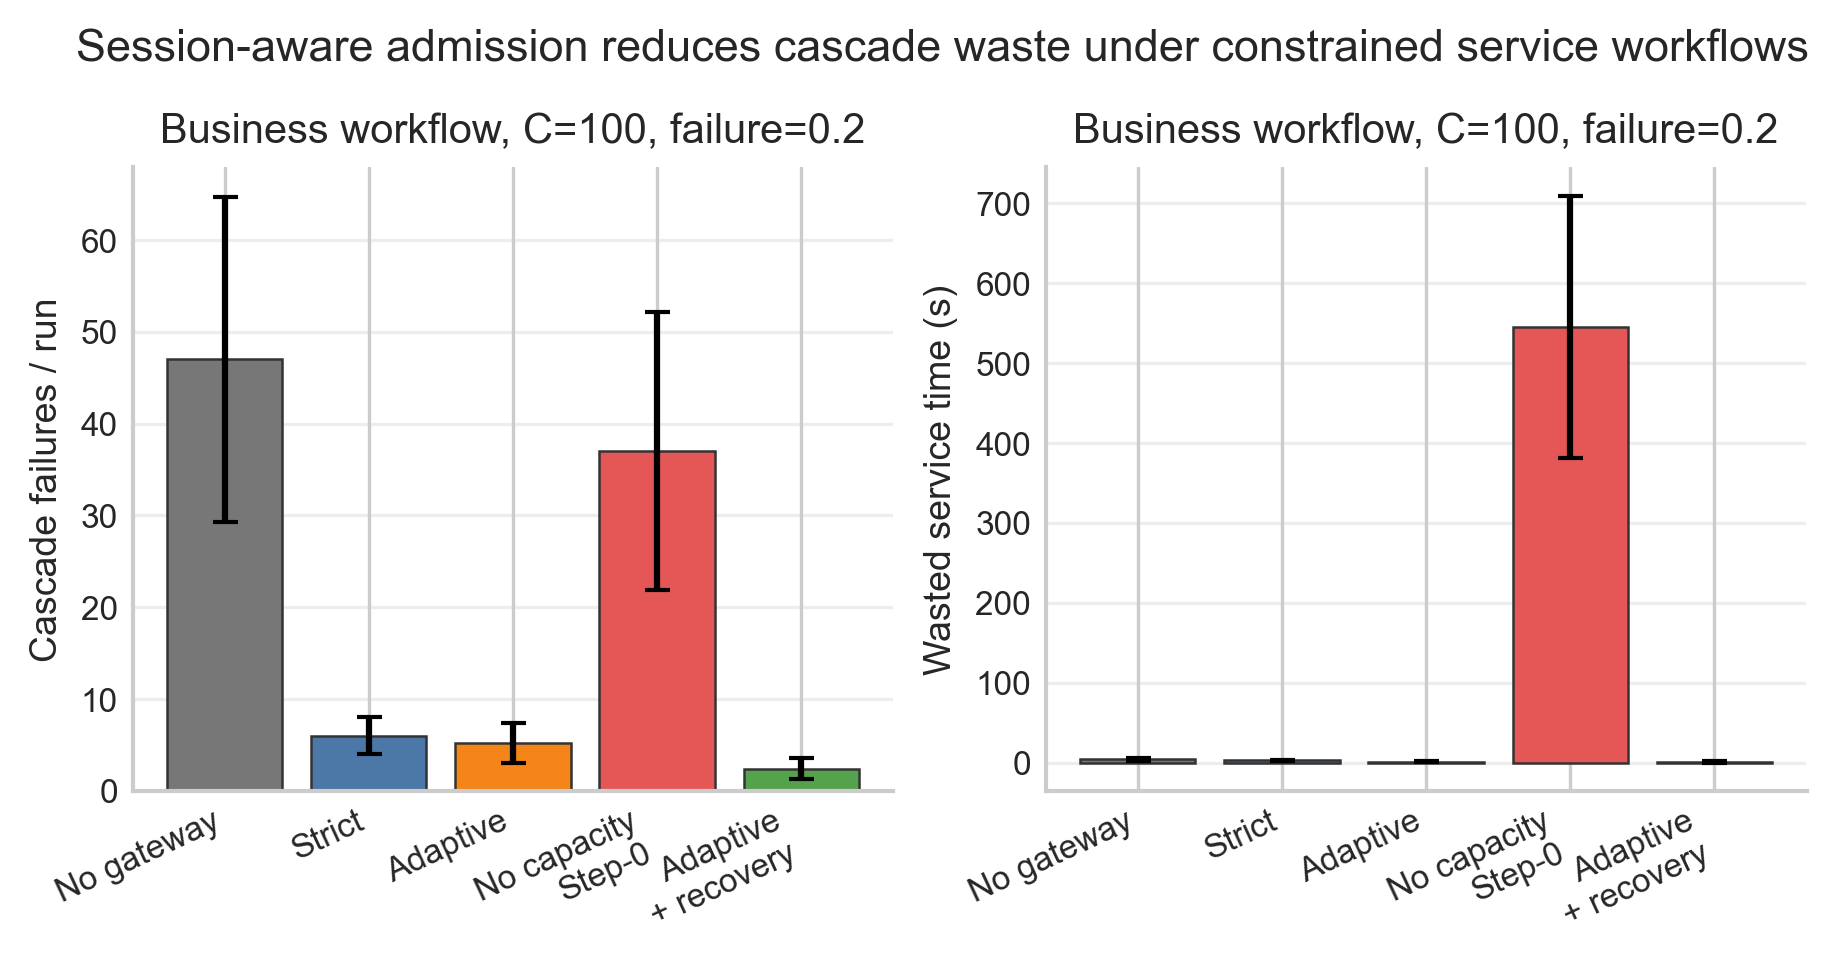
\includegraphics[width=0.84\textwidth]{fig_jss_core_tradeoff.png}
\caption{Core service-workflow trade-off. Adaptive admission reduces cascade and wasted service time under constrained business-workflow load; the result concerns waste governance rather than raw-success ranking.}
\label{fig:jss_core_tradeoff}
\end{figure*}

This result supports RQ1 with an important scope condition. In the same setting, raw workflow success is not the primary optimization target and may differ across policies. We therefore read the result as waste-governance support: when backend capacity and failures make admitted-but-doomed sessions likely, session-aware capacity admission reduces cascade waste and wasted service time.

\subsection{RQ2: Adaptive Admission Trade-Off}

RQ2 asks whether capacity admission should be fixed or pressure-aware. The constrained business-workflow result in RQ1 shows one side of the trade-off: removing capacity step-0 rejection creates more cascade and wasted service time under high-load failure conditions. Strict admission captures the opposite risk: rejecting early can deny work that might have completed when the backend has headroom. Adaptive admission keeps hard rejection but changes only the capacity gate according to pressure signals.

The cloud-backend smoke test shows the other side of the trade-off. In the single-repeat cloud-provider setting, no-capacity-step0 exceeds adaptive by 7 successful sessions. This is a descriptive scope result rather than a global ranking: provider elasticity can absorb load that the local gateway would otherwise reject. Figure~\ref{fig:jss_backend_boundary} summarizes this backend-dependent interpretation.

\begin{figure*}[t]
\centering
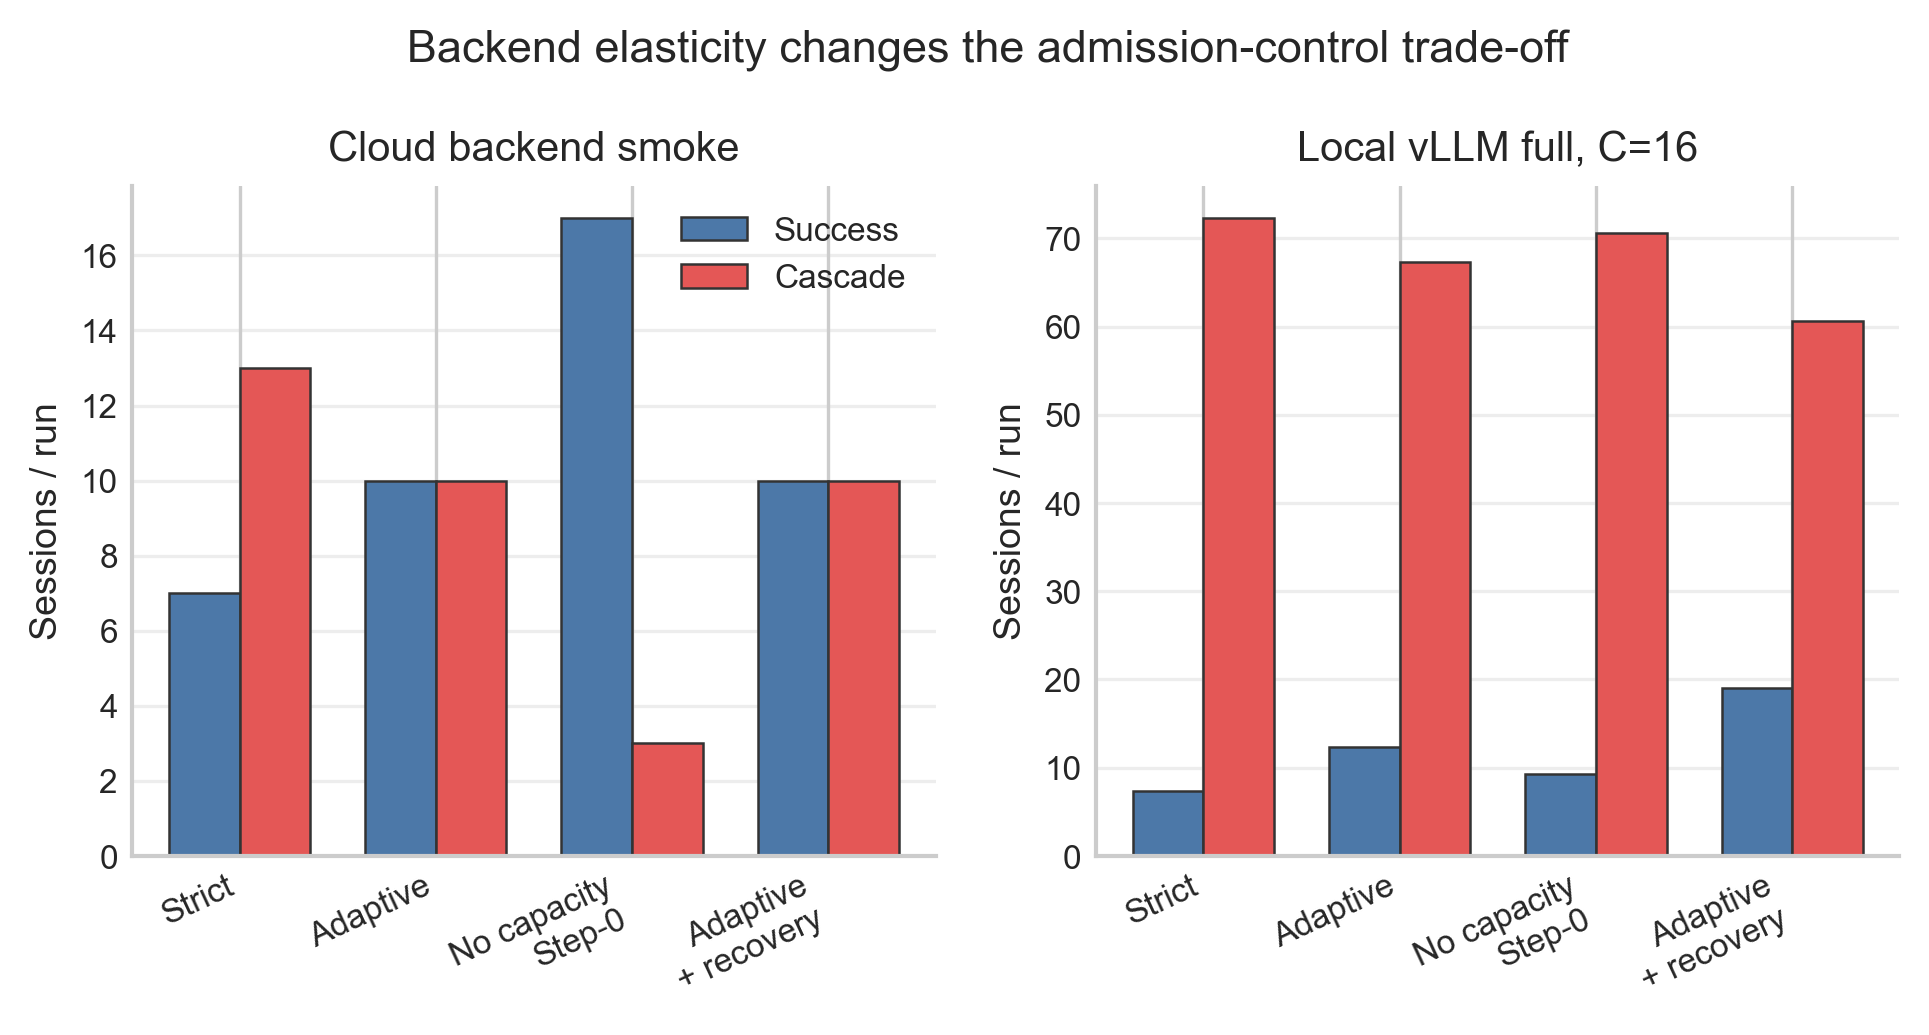
\includegraphics[width=0.84\textwidth]{fig_jss_backend_boundary.png}
\caption{Backend-dependent admission scope. Constrained backends and elastic providers can favor different raw-success trade-offs, so provider results are interpreted descriptively rather than as a universal policy ranking.}
\label{fig:jss_backend_boundary}
\end{figure*}

\subsection{RQ3: ReAct Recovery and Side-Effect Safety}

Client-cooperative recovery improves recovered progress without turning the gateway into an automatic replay engine. In the core business-workflow setting at $C{=}100,F{=}0.2$, adaptive-react-recovery increases recovered ReAct sessions by 2.4 relative to adaptive admission alone, with confidence interval $[0.8,4.0]$. It also increases avoided replay steps by 10.0, with confidence interval $[1.6,19.6]$.

The targeted vLLM recovery arm provides model-backed feasibility evidence. At $C{=}2$, the recovery variant increases recovered sessions by 9.33 relative to adaptive, with confidence interval $[8.0,10.0]$. This arm uses a hybrid setup with a DeepSeek agent brain and a local Qwen vLLM backend, so it should not be merged with natural full-vLLM recovery claims. Figure~\ref{fig:jss_recovery_effectiveness} summarizes the recovery results.

\begin{figure*}[t]
\centering
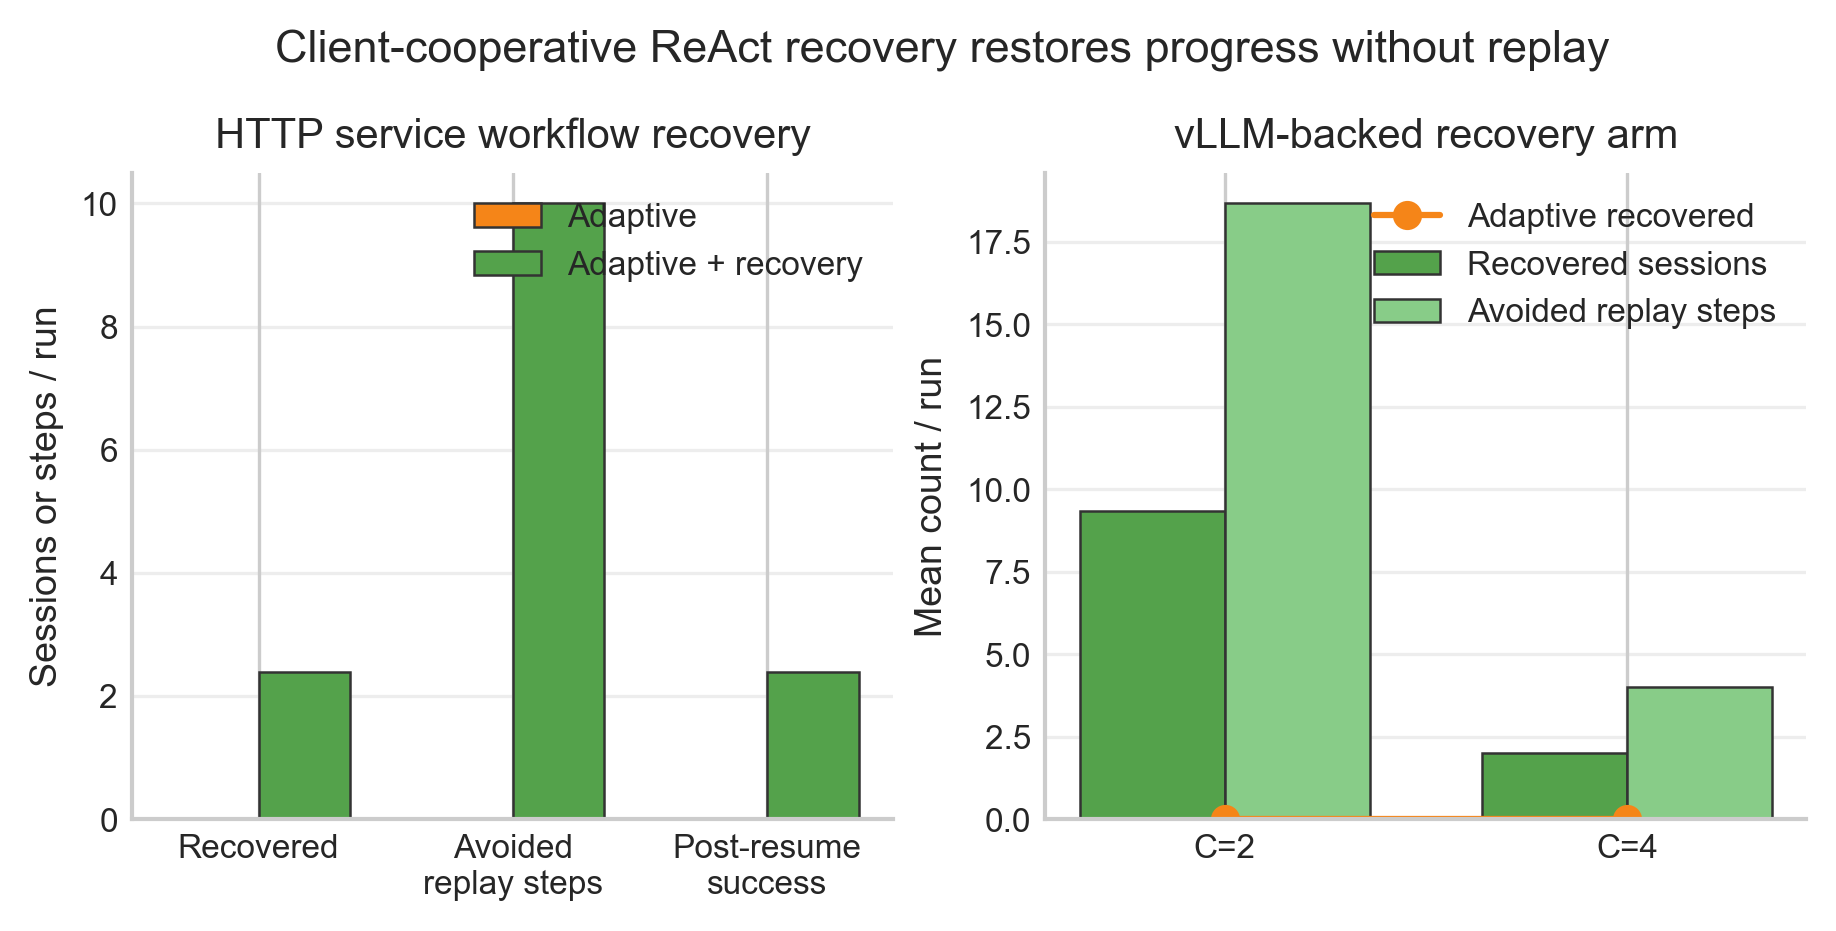
\includegraphics[width=0.84\textwidth]{fig_jss_recovery_effectiveness.png}
\caption{Client-cooperative ReAct recovery. Recovery restores checkpointed progress and avoids replayed steps, but it does not execute future tools on behalf of the client.}
\label{fig:jss_recovery_effectiveness}
\end{figure*}

Protocol-level checks support the same scope. The recovery protocol passes 11/11 declared edge cases, including no automatic future-tool execution and duplicate-side-effect checks. The E2E correctness smoke contains 9 summary rows with empty validation errors. The E2E performance-sanity set contains 18 runs over $C\in\{10,20\}$, zero duplicate side effects, and consistent database state in 18/18 rows. These checks support side-effect correctness and recovery usability, not real-service performance ranking.

\subsection{RQ4: Deployability, Overhead, and Sensitivity}

The operator-overhead study indicates that \plangate's steady-state overhead is modest in the tested gateway path. At $C{=}100$, adaptive versus baseline has a small negative p95 latency delta in this run, approximately $-6.37$ ms, while the throughput delta confidence interval crosses zero. We interpret this as no large overhead under the tested gateway path, not as a general latency-reduction result.

The configuration-sensitivity study shows that governance parameters affect recovery strength. Under $C{=}100,F{=}0.2$, a strict-versus-default recovery-sensitivity comparison changes recovered sessions by $-1.67$. This supports qualitative robustness and sensitivity analysis, not selection of a globally optimal configuration. Component mapping records 9 architecture components mapped to 18 result records, which is used to organize the design rationale rather than to argue that every component improves raw success. Figure~\ref{fig:jss_overhead_sensitivity} summarizes overhead and sensitivity results.

\begin{figure*}[t]
\centering
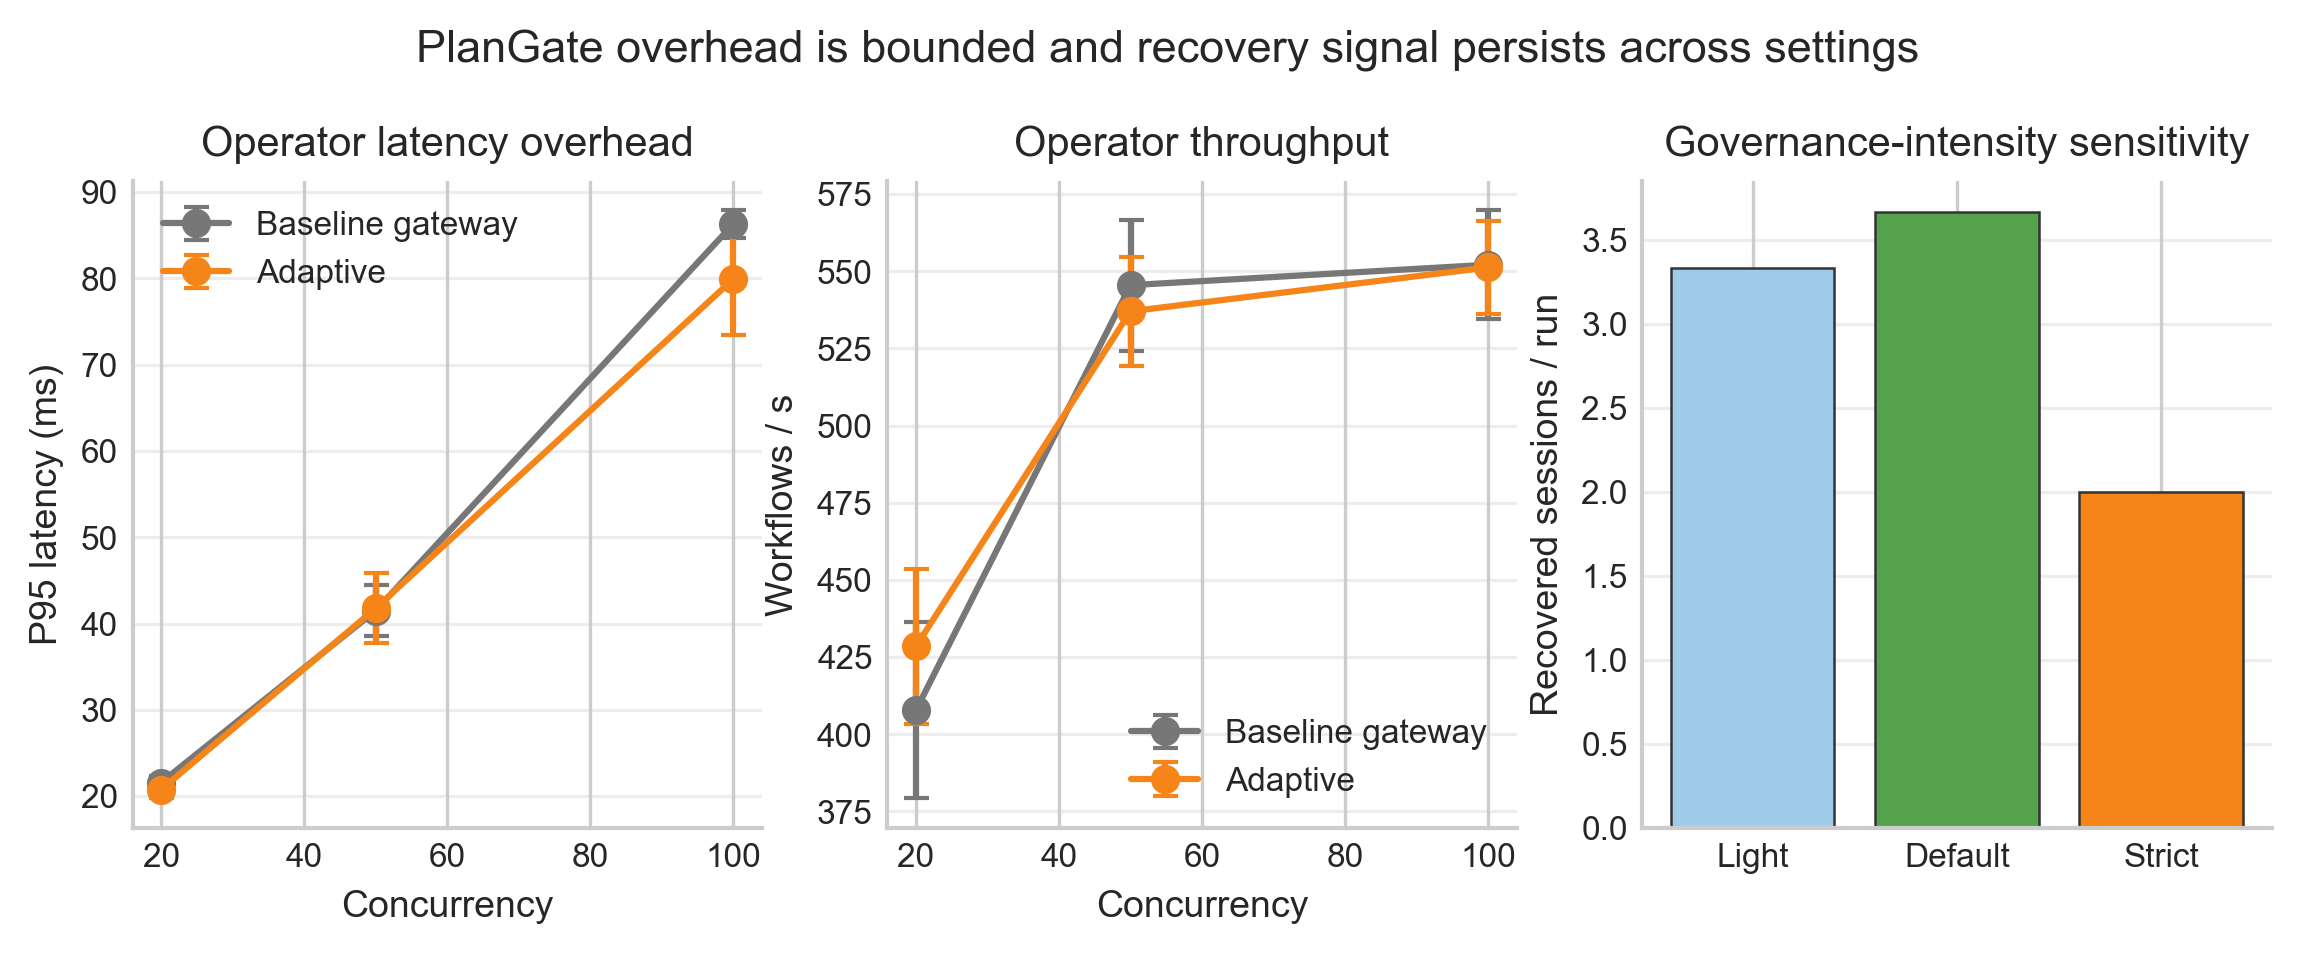
\includegraphics[width=0.84\textwidth]{fig_jss_overhead_sensitivity.png}
\caption{Deployability results. Operator overhead is modest in the tested path, while configuration sensitivity shows that recovery strength depends on governance settings.}
\label{fig:jss_overhead_sensitivity}
\end{figure*}

\subsection{RQ5: External Validity and Distributed Correctness}

The real-service and distributed studies provide the main external-validity support. The HTTP+SQLite checks show that MCP tools call external HTTP services, side effects are persisted, idempotency prevents duplicate writes, and recovery can resume without replaying completed operations. These runs are treated as correctness and sanity checks rather than the main performance setting.

The clean CloudLab distributed result is the deterministic correctness probe. CloudLab provides scientific infrastructure for controlled cloud-architecture experiments \citep{ricci2014cloudlab}. In our six-node deployment, Redis-backed shared state recovers 15/15 forced cross-gateway ReAct resumes with zero state misses, while the memory-local diagnostic control misses 15/15 forced cross-gateway resumes. Replayed completed side effects are zero. Figure~\ref{fig:cloudlab_deployment_topology} shows the deployment topology, and Figure~\ref{fig:jss_distributed_correctness} shows the distributed correctness result.

\begin{figure*}[t]
\centering
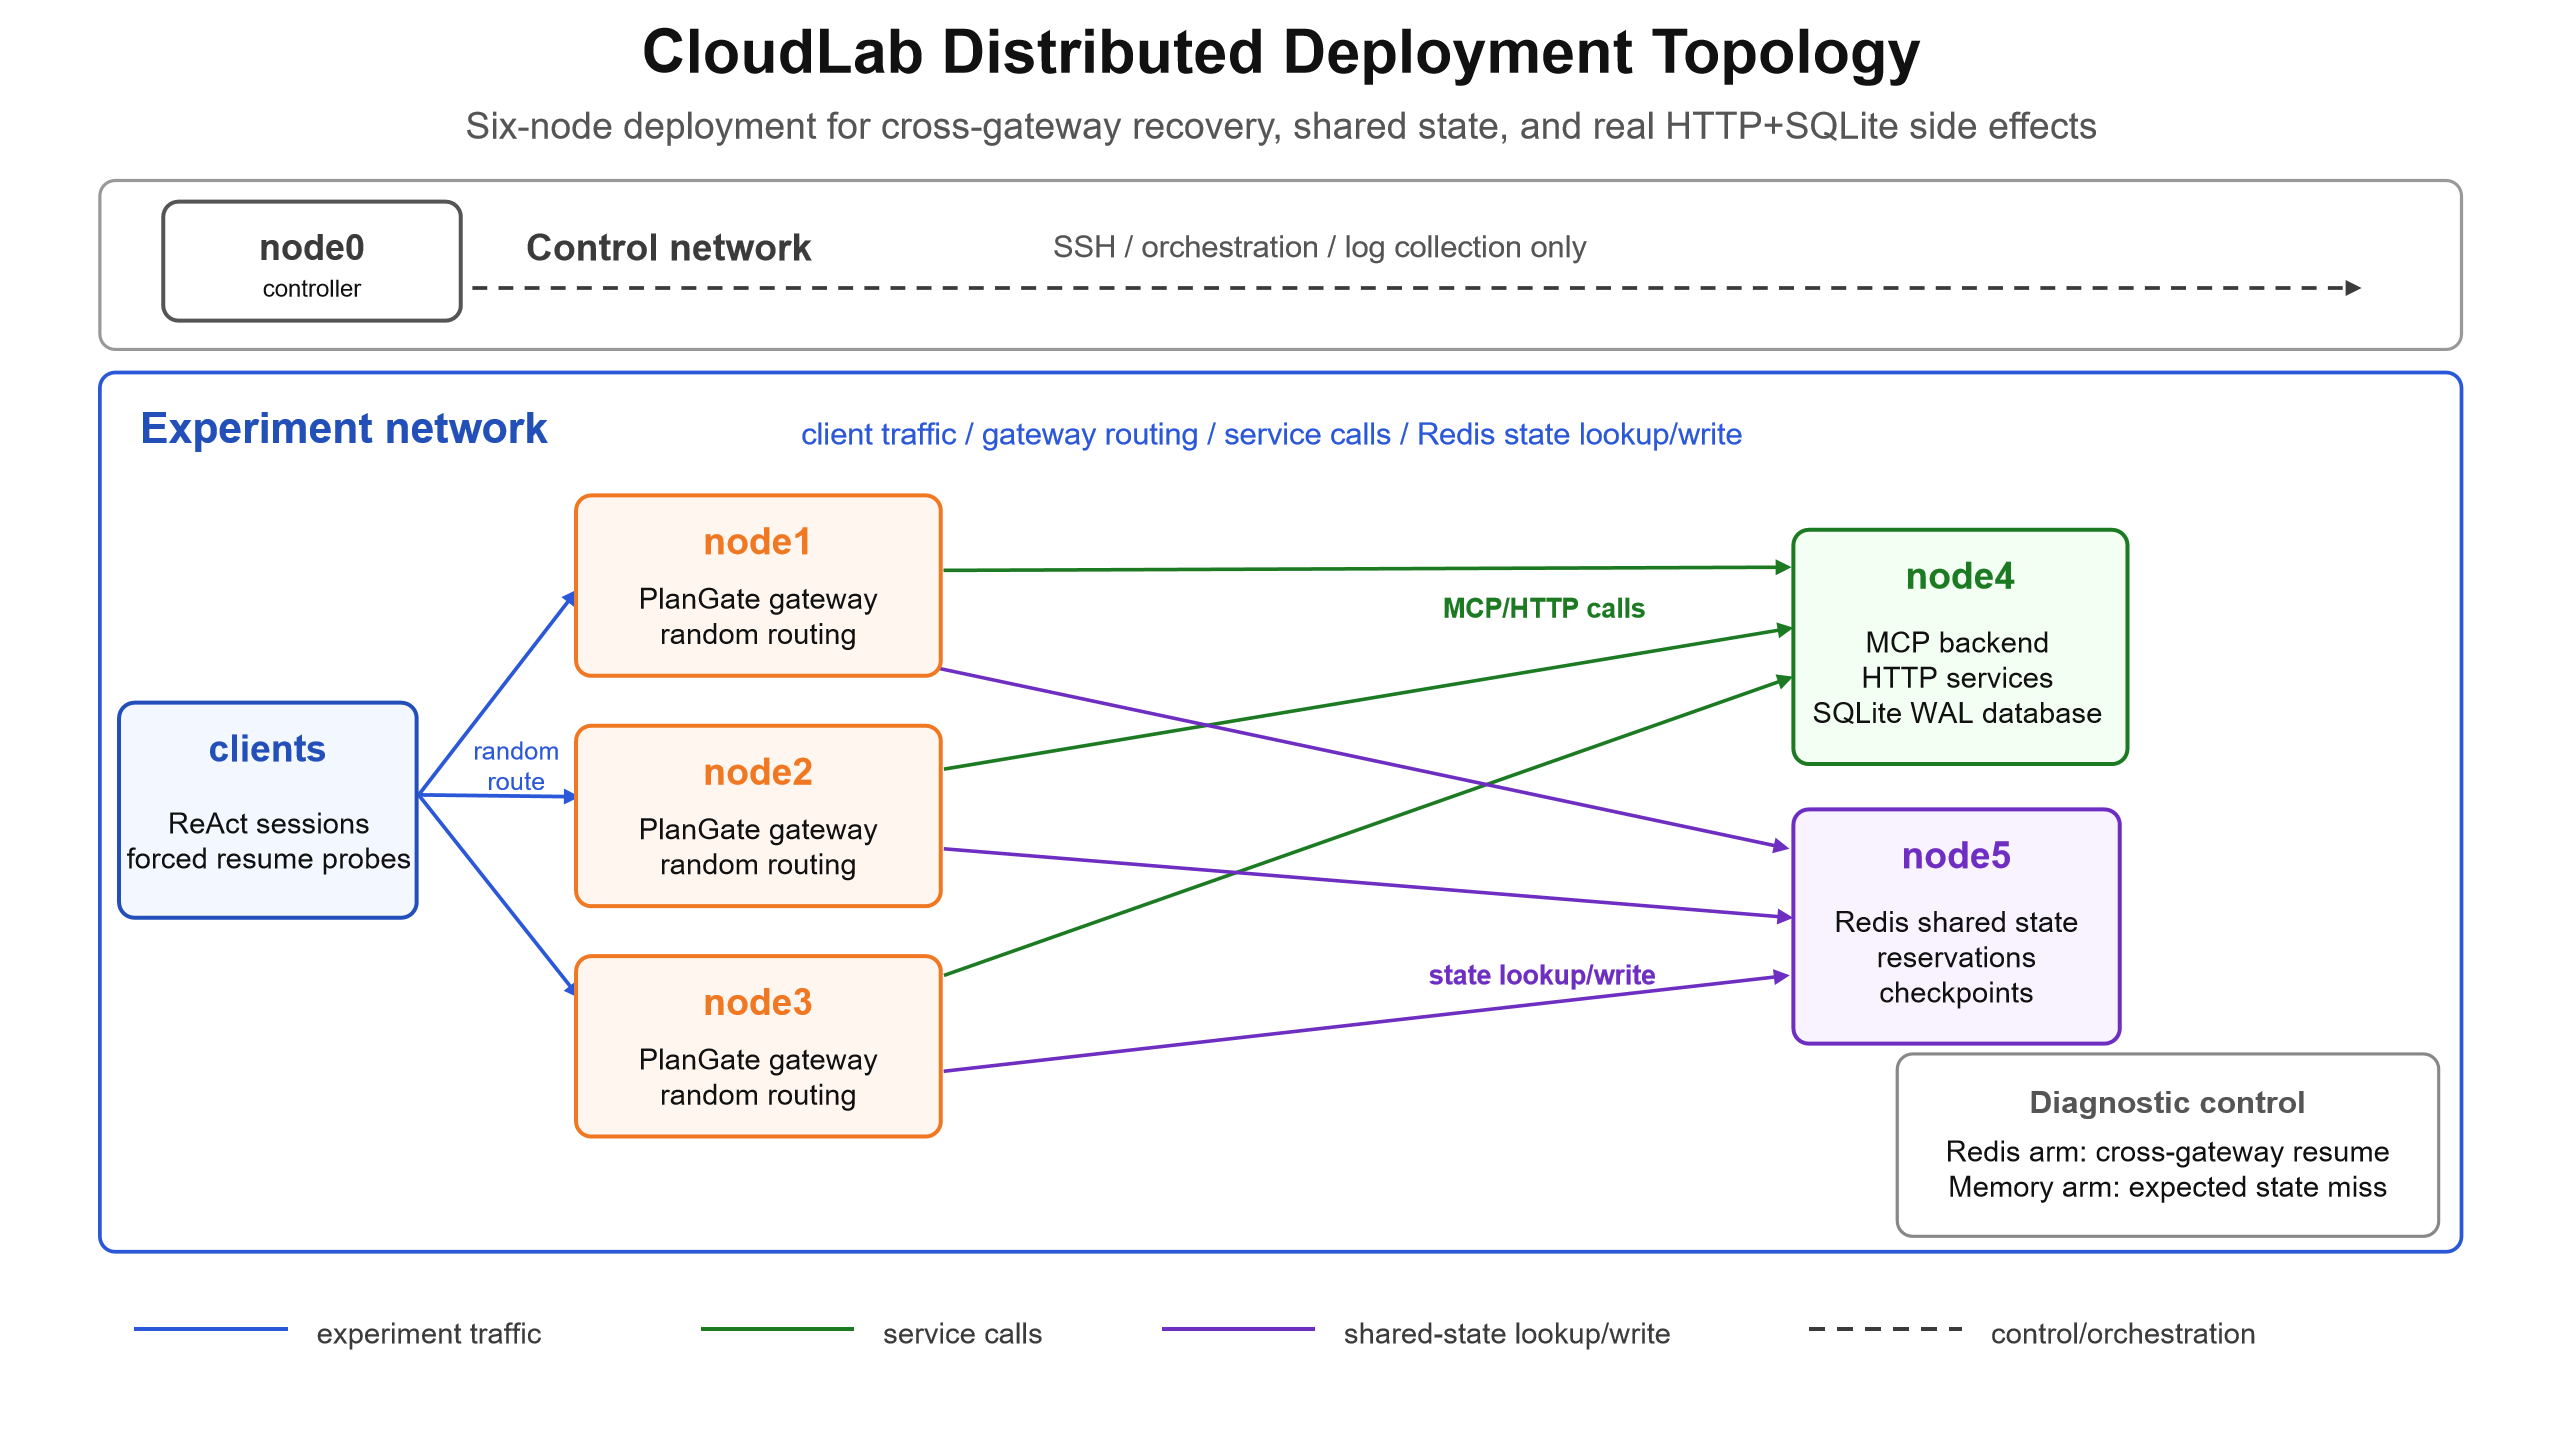
\includegraphics[width=0.88\textwidth]{fig_cloudlab_deployment_topology.png}
\caption{CloudLab distributed deployment topology used for the deterministic correctness probe. Multiple gateways route to external business services, while Redis and memory-local state are compared as shared-state and diagnostic arms.}
\label{fig:cloudlab_deployment_topology}
\end{figure*}

\begin{figure*}[t]
\centering
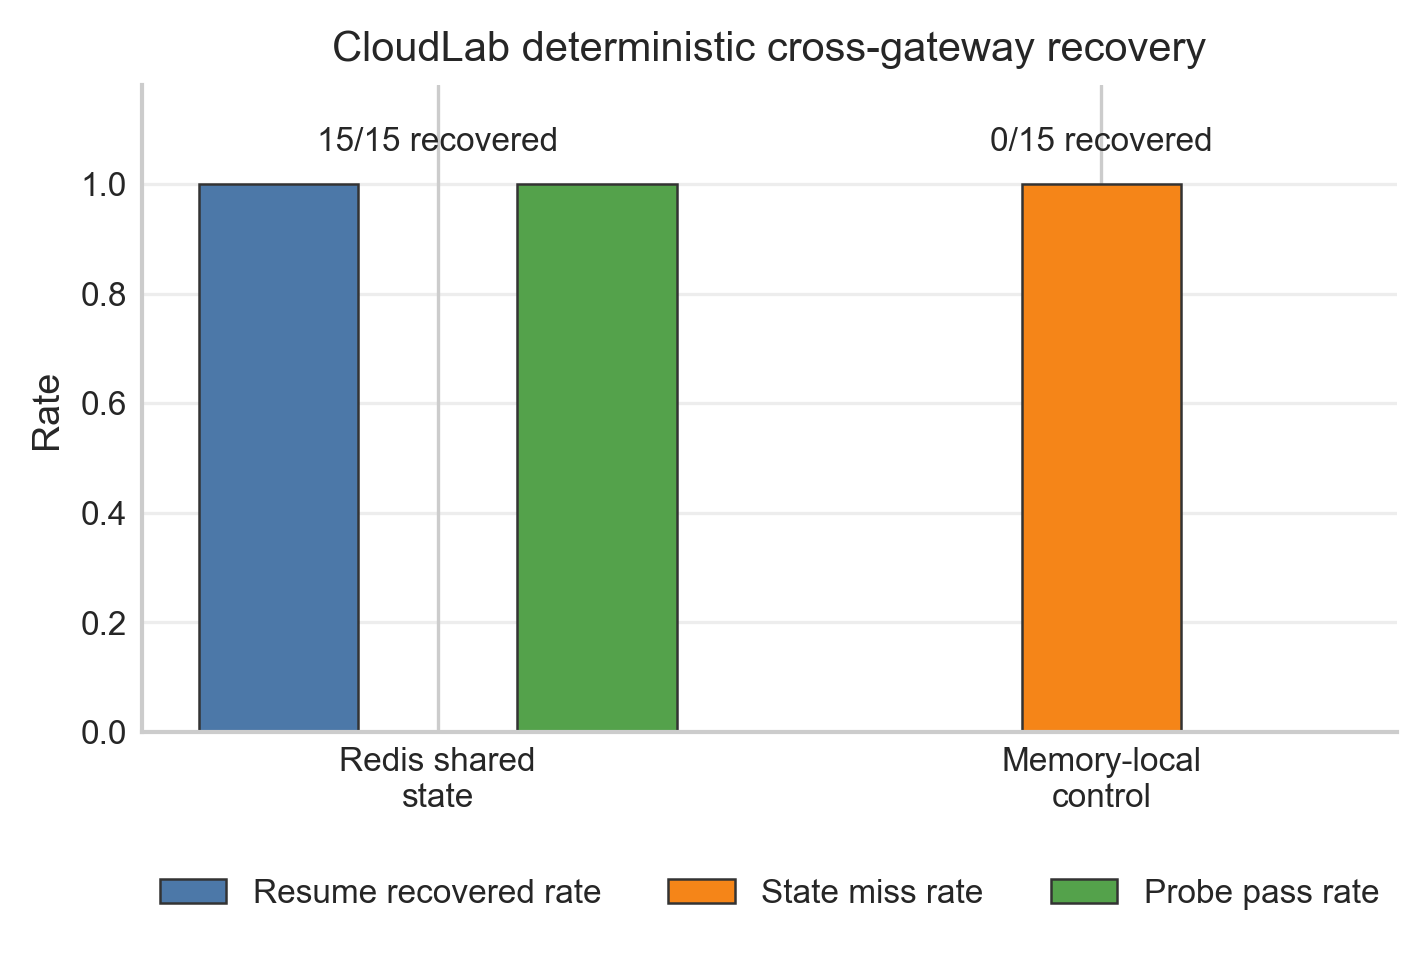
\includegraphics[width=0.84\textwidth]{fig_jss_distributed_correctness.png}
\caption{Distributed correctness on CloudLab. Redis-backed shared state supports forced cross-gateway recovery; memory-local state misses cross-gateway checkpoints. This checks shared-state necessity, not production Redis HA.}
\label{fig:jss_distributed_correctness}
\end{figure*}

An earlier CloudLab distributed probe provides supporting context: Redis recovered 9/9 forced cross-gateway resumes, while memory-local state missed 9/9. The deterministic study supersedes this earlier mixed random-workload run for the main distributed-correctness result because the earlier random workload rows include expected ACTIVE\_CHECKPOINT conflicts.

\subsection{Workflow Shape, Arrival Realism, and Cross-Layer Smoke}

Supporting studies address representativeness and execution stability. A metadata-derived MCP-Bench smoke selects 30 tasks and executes without errors, supporting workflow-shape diversity rather than full MCP-Bench deployment or model-accuracy conclusions. A BurstGPT-shaped replay covers normal, burst, and peak-burst windows with scale factors 1.0, 1.5, and 2.0, supporting arrival-pattern realism while keeping session structure controlled. The cross-layer smoke index covers mock, cloud LLM, and vLLM layers with empty validation errors. These studies support generality and stability, not headline performance rankings.

\begin{table*}[t]
\centering
\caption{Main JSS results and interpretation scope.}
\label{tab:main_results_summary}
\footnotesize
\begin{tabular}{@{}>{\raggedright\arraybackslash}p{0.22\textwidth}>{\raggedright\arraybackslash}p{0.39\textwidth}>{\raggedright\arraybackslash}p{0.29\textwidth}@{}}
\toprule
\textbf{Role} & \textbf{Supported result} & \textbf{Scope} \\
\midrule
Core service workflow & Adaptive reduces cascade by 31.8 and wasted service time by about 544,149 ms at $C{=}100,F{=}0.2$. & Not a raw-success ranking. \\
Client-cooperative recovery & Recovery adds 2.4 recovered sessions and 10.0 avoided replay steps in the core workflow. & Does not auto-execute future tools. \\
Real-backend recovery & vLLM recovery arm adds 9.33 recovered sessions at $C{=}2$. & Targeted hybrid arm, not natural full-vLLM recovery. \\
E2E side-effect correctness & HTTP+SQLite sanity records zero duplicate side effects and consistent DB state in 18/18 rows. & Small sanity, not main performance benchmark. \\
Distributed correctness & CloudLab Redis recovers 15/15 forced cross-gateway resumes; memory misses 15/15. & No production Redis HA claim. \\
Provider scope & Cloud backend smoke shows no-capacity can exceed adaptive by 7 successes. & Single-repeat descriptive result. \\
\bottomrule
\end{tabular}
\end{table*}

\section{Discussion}
\label{sec:discussion}

\subsection{Why Session-Aware Governance Helps}

The results support the paper's central claim: request-level governance is insufficient for dependent agent workflows. When capacity is constrained, admitting a session that later fails wastes completed tool calls and service time. Adaptive capacity admission reduces this waste by moving some unavoidable rejection earlier while preserving hard rejection for invalid workflows. Recovery contributes a second benefit: it restores a safe point without making the gateway an autonomous agent or replay engine.

\subsection{When Admission Control Can Hurt}

The provider-backed results show that admission control is not universally beneficial. Elastic cloud providers can hide queueing pressure, absorb load bursts, and make no-capacity-step0 look better in raw success. This defines the deployment scope: \plangate is most valuable when backend capacity is constrained, shared, costly, or stateful. When a provider absorbs overload externally, the gateway should use provider-aware signals rather than enforce a fixed local capacity rule.

\subsection{Distributed State as a Correctness Requirement}

The CloudLab results show that shared state is not merely an optimization. Cross-gateway resume requires checkpoint availability beyond a single process. The memory-local diagnostic control fails exactly where expected: it cannot find checkpoints created on another gateway. Redis-backed state fixes this lookup problem in the tested deployment. The result should still be read narrowly. It validates shared-state necessity for checkpoint and reservation lookup; it does not claim production Redis high availability, crash recovery, or replicated control-plane fault tolerance.

\subsection{Implications for Service Workflow Engineering}

The broader implication is that LLM-agent infrastructure should expose workflow semantics to the gateway layer. Session identifiers, step indexes, idempotency keys, recovery modes, and declared-plan metadata are not incidental annotations. \plangate turns this metadata into an operational control contract through which the gateway can reason about cascade waste, continuation value, side-effect safety, and distributed recovery.

\section{Threats to Validity}
\label{sec:threats}

\subsection{Internal Validity}

The controlled experiments use repeated runs and fixed configurations, but they still depend on implementation choices in the runners and failure injectors. Bugs in clients, validators, or aggregation scripts could affect the results. To reduce this risk, the package includes run metadata, bootstrap/effect summaries, scoped finding tables, and a lightweight replay validator. Unit tests cover recovery semantics and session-cap behavior, but they do not eliminate all implementation risk.

\subsection{Construct Validity}

Metrics such as cascade failure, wasted service time, avoided replay steps, duplicate side effects, and state miss are proxies for service-workflow governance quality. They capture the paper's main failure modes, but they do not capture all possible user-facing outcomes. For example, raw workflow success can be lower under admission control even when cascade waste is lower. The paper therefore avoids interpreting all metrics as a single scalar utility.

\subsection{Client Cooperation and Metadata Validity}

\plangate relies on client-provided workflow metadata, including session identifiers, step indexes, idempotency keys, and recovery modes. The evaluation checks malformed metadata and recovery edge cases, but it does not cover a complete adversarial-client model. A client that omits metadata, reuses identifiers incorrectly, or intentionally lies about workflow state can weaken the governance contract. This threat is inherent in making workflow metadata part of the operational interface.

\subsection{External Validity}

The evaluation covers controlled business workflows, mock backends, vLLM, cloud-provider smoke tests, HTTP+SQLite services, MCP-Bench-derived workflow shapes, BurstGPT-shaped arrival replay, and CloudLab distributed deployment. This is broader than a single benchmark, but it is not a production deployment study. The CloudLab experiments are correctness probes rather than long-running production workloads. The BurstGPT-shaped replay uses real LLM-serving arrival structure, but session structure remains controlled. Cloud-provider behavior may vary across time, region, quota, and provider policy.

\subsection{Reproducibility Threats}

Some experiments depend on external cloud providers and local vLLM deployment, which can be sensitive to model versions, rate limits, and hardware. AI-enabled software systems can accumulate hidden dependencies and operational technical debt, so uncontrolled provider changes are a real reproducibility threat \citep{sculley2015technicaldebt}. The artifact addresses this by separating controlled studies from provider-scope smoke tests and by recording run metadata. The lightweight replay validator checks internal consistency of the submitted package, but full reruns may still require provider credentials, CloudLab resources, or local model-serving setup.

\subsection{Cost-Model Validity}

Wasted service time and token use are proxy costs. They are useful for comparing policies under controlled settings, but they do not directly equal provider billing, user-perceived utility, or business value. The paper therefore treats cost-related metrics as operational waste indicators rather than a complete economic model.

\section{Related Work}
\label{sec:related_work}

\subsection{LLM Agent Tool Use and MCP Workflows}

Tool-using LLM research studies how models select tools, call APIs, and solve multi-step tasks. ReAct interleaves reasoning traces and actions \citep{yao2023react}; Toolformer studies how language models can learn when and how to call tools \citep{schick2023toolformer}; ToolBench and Gorilla-style work evaluate large API/tool ecosystems \citep{qin2024toolbench,patil2023gorilla}. These systems and benchmarks are essential for measuring whether an agent chooses the right tool and supplies the right arguments. \plangate addresses a different layer: it governs the service workflow after tool calls are issued. Its focus is admission, continuation, recovery, idempotency, and distributed state rather than model reasoning accuracy.

Recent agent benchmarks also show why gateway-level governance is needed. WebArena and OSWorld evaluate agents in realistic browser or computer environments \citep{zhou2023webarena,xie2024osworld}. $\tau$-bench models user-agent-tool interaction in business domains, and MCP-Bench connects agents to live MCP servers and hundreds of tools \citep{taubench2024,mcpbench2025}. These benchmarks emphasize task completion and tool-use competence. In this paper, they motivate workflow-shape smoke tests, but they are not the main performance substrate. The core claim is about infrastructure governance under constrained or shared backends, not about agent task accuracy.

MCP standardizes the connection between model applications and external tools \citep{anthropic2024mcp}. This standardization makes the gateway position especially important: the gateway can observe tool calls, session metadata, and backend outcomes without modifying the model. \plangate uses this position to enforce session-aware governance, but it does not require a new agent framework or model-specific tool-use training.

\subsection{Service Workflows and Runtime Governance}

Traditional service workflow systems reason about orchestration, compensation, state, and reliability across dependent service calls. Service-oriented computing frames services as composable software units and identifies composition, coordination, and management as core research concerns \citep{papazoglou2003soc,papazoglou2008roadmap}. Saga-style transactions define long-lived activities and compensating actions \citep{garciamolina1987sagas}. Workflow research and workflow-pattern studies characterize recurring control-flow, synchronization, and exception-handling structures in service processes \citep{vanderAalst2003workflowpatterns}. These systems often assume an explicit workflow specification or an orchestration engine. \plangate is lighter weight: it does not introduce a new workflow language and does not require all agents to submit a complete workflow graph. Instead, it uses metadata available at the gateway to govern admission, continuation, and recovery for agent-generated service calls.

API gateways, load balancers, rate limiters, and overload controllers protect backend services by shaping request traffic. Classical server overload work, staged event-driven architectures, autonomic management, and queue-management mechanisms show that runtime policy must account for queueing, backpressure, and adaptation \citep{welsh2001seda,kephart2003autonomic,nichols2012codel}. Auto-scaling surveys similarly show that resource policies depend on workload, SLA, and elasticity assumptions \citep{lorido2014autoscaling}. These systems usually treat requests, queues, or resource pools as the control unit. \plangate differs by making the session the governance unit: late-step rejection has a different cost from new-session rejection, and recovery must account for completed side-effecting steps. This is the gap that motivates session-aware governance.

Microservice research highlights independently deployable services, distributed service interactions, and operational complexity \citep{dragoni2017microservices}. Benchmarks such as DeathStarBench and TeaStore provide production-like service graphs for studying latency, resource management, and service interactions \citep{gan2019deathstarbench,vonkistowski2018teastore}. \plangate is complementary. It does not replace microservice resource management; instead, it governs LLM-agent workflows that call tools and services, including model-backed and side-effecting services.

\subsection{LLM Serving and Backend Overload}

LLM serving systems study batching, scheduling, caching, and inference throughput. Orca introduces iteration-level scheduling for transformer serving, vLLM uses PagedAttention to improve memory management, and FastServe explores distributed inference scheduling for LLMs \citep{yu2022orca,kwon2023vllm,wu2023fastserve}. These systems are complementary to \plangate. A serving system decides how to execute model requests efficiently; \plangate decides whether and how a multi-step workflow should be admitted, continued, or recovered across tools and services that may include model-backed calls. The vLLM experiments in this paper use local model serving as a constrained backend, but the mechanism is gateway-level and backend-agnostic.

Trace-based LLM-serving studies such as BurstGPT show that model-serving traffic can be bursty and session-shaped \citep{wang2024burstgpt}. Tail-latency studies also show that queueing and fan-out effects can dominate perceived service performance at scale \citep{dean2013tail}. \plangate uses trace-shaped replay as supporting arrival-realism evidence, but it does not claim to possess a production agent trace. Cloud LLM providers add another layer: hidden queues, elastic headroom, rate limits, and provider-specific failure behavior. The provider-boundary results show that policies tuned for local constrained backends may not maximize raw success under elastic providers. This observation aligns with service-management work that treats runtime policy as environment-dependent rather than fixed.

\subsection{Recovery, Idempotency, and Distributed State}

Distributed systems commonly use checkpointing, idempotency, leases, durable logs, and shared state to handle failures. Chandy-Lamport snapshots define a classic basis for consistent distributed-state observation \citep{chandy1985distributed}. Leases provide time-bounded coordination \citep{gray1989leases}; ZooKeeper provides coordination primitives for distributed systems \citep{hunt2010zookeeper}; Dynamo and Raft illustrate different approaches to availability and consensus in distributed storage and replication \citep{decandia2007dynamo,ongaro2014raft}. \plangate does not attempt to solve full distributed consensus or replicated storage. It uses shared state narrowly for reservation and checkpoint lookup across gateways.

Service systems also rely on idempotency keys and stable operation identifiers to make retries safe. HTTP semantics distinguish safe and idempotent operations, but practical workflows still require application-level identifiers for durable side effects \citep{rfc9110}. \plangate applies these ideas to LLM-agent service workflows, where the failure boundary is complicated by online tool choice and side-effecting operations.

The recovery protocol is deliberately client-cooperative because future tool choice belongs to the agent client. Redis-backed state is used to make checkpoints available across gateway processes, while the paper avoids claims about production-grade high availability. This positions \plangate between stateless API gateways and full workflow engines: it adds enough session state to govern agent workflows without taking over the agent's planning role.

\subsection{Positioning Summary}

Table~\ref{tab:related_positioning} summarizes the distinction between \plangate and adjacent research lines. The common theme is that prior work either evaluates the agent, optimizes the backend, orchestrates explicit workflows, or provides distributed coordination. \plangate instead targets gateway-level governance for multi-step service workflows after tool calls are issued but before their execution and recovery semantics become unsafe.

\begin{table}[t]
\centering
\caption{Positioning of PlanGate relative to adjacent research lines.}
\label{tab:related_positioning}
\footnotesize
\begin{tabular}{@{}>{\raggedright\arraybackslash}p{0.25\columnwidth}>{\raggedright\arraybackslash}p{0.32\columnwidth}>{\raggedright\arraybackslash}p{0.34\columnwidth}@{}}
\toprule
\textbf{Line of work} & \textbf{Primary focus} & \textbf{Gap addressed by PlanGate} \\
\midrule
Agent/tool benchmarks & Tool choice and task success. & Gateway-level workflow governance after tool calls are issued. \\
LLM serving & Efficient model-request execution. & Session admission, continuation, and recovery across tools. \\
Workflow engines & Explicit orchestration and compensation. & Lightweight governance for agent-generated MCP workflows. \\
Distributed state & Coordination and storage correctness. & Cross-gateway checkpoint availability for agent sessions. \\
\bottomrule
\end{tabular}
\end{table}

\section{Conclusion}
\label{sec:conclusion}

This paper presented \plangate, a session-aware governance gateway for multi-step LLM service workflows. The central observation is that request-level governance does not match dependent agent sessions: rejecting a late tool call can waste earlier work and risk unsafe replay. \plangate addresses this mismatch with session-aware admission, client-cooperative recovery, idempotency, and optional Redis-backed shared state.

The evaluation shows that adaptive governance reduces cascade and wasted service time under constrained business-workflow load, ReAct recovery restores checkpointed progress without server-side replay, and HTTP+SQLite and CloudLab studies validate side-effect and distributed-state correctness. The results also define a deployment scope: elastic cloud providers can invert admission-control trade-offs. \plangate should therefore be read as a workflow-governance framework for constrained, shared, or stateful service backends, not as a universally dominant admission policy.

\begin{thebibliography}{99}

\bibitem[Anthropic(2024)]{anthropic2024mcp}
Anthropic.
\newblock Model Context Protocol.
\newblock \url{https://modelcontextprotocol.io/}, 2024.

\bibitem[Chandy and Lamport(1985)]{chandy1985distributed}
K. M. Chandy and L. Lamport.
\newblock Distributed snapshots: Determining global states of distributed systems.
\newblock \emph{ACM Transactions on Computer Systems}, 3(1):63--75, 1985.

\bibitem[DeCandia et~al.(2007)]{decandia2007dynamo}
G. DeCandia, D. Hastorun, M. Jampani, G. Kakulapati, A. Lakshman, A. Pilchin, S. Sivasubramanian, P. Vosshall, and W. Vogels.
\newblock Dynamo: Amazon's highly available key-value store.
\newblock In \emph{Proceedings of SOSP}, 2007.

\bibitem[Dean and Barroso(2013)]{dean2013tail}
J. Dean and L. A. Barroso.
\newblock The tail at scale.
\newblock \emph{Communications of the ACM}, 56(2):74--80, 2013.

\bibitem[Dragoni et~al.(2017)]{dragoni2017microservices}
N. Dragoni, S. Giallorenzo, A. L. Lafuente, M. Mazzara, F. Montesi, R. Mustafin, and L. Safina.
\newblock Microservices: Yesterday, today, and tomorrow.
\newblock In M. Mazzara and B. Meyer (Eds.), \emph{Present and Ulterior Software Engineering}, pp. 195--216. Springer, 2017.

\bibitem[Gan et~al.(2019)]{gan2019deathstarbench}
Y. Gan, Y. Zhang, K. Hu, D. Cheng, Y. He, M. Pancholi, and C. Delimitrou.
\newblock An open-source benchmark suite for microservices and their hardware-software implications for cloud and edge systems.
\newblock In \emph{Proceedings of ASPLOS}, 2019.

\bibitem[Garcia-Molina and Salem(1987)]{garciamolina1987sagas}
H. Garcia-Molina and K. Salem.
\newblock Sagas.
\newblock In \emph{Proceedings of ACM SIGMOD}, 1987.

\bibitem[Gray and Cheriton(1989)]{gray1989leases}
C. Gray and D. Cheriton.
\newblock Leases: An efficient fault-tolerant mechanism for distributed file cache consistency.
\newblock In \emph{Proceedings of SOSP}, 1989.

\bibitem[Hunt et~al.(2010)]{hunt2010zookeeper}
P. Hunt, M. Konar, F. P. Junqueira, and B. Reed.
\newblock ZooKeeper: Wait-free coordination for Internet-scale systems.
\newblock In \emph{Proceedings of USENIX ATC}, 2010.

\bibitem[Kephart and Chess(2003)]{kephart2003autonomic}
J. O. Kephart and D. M. Chess.
\newblock The vision of autonomic computing.
\newblock \emph{Computer}, 36(1):41--50, 2003.

\bibitem[Kwon et~al.(2023)]{kwon2023vllm}
W. Kwon, Z. Li, S. Zhuang, Y. Sheng, L. Zheng, C. H. Yu, J. E. Gonzalez, H. Zhang, and I. Stoica.
\newblock Efficient memory management for large language model serving with PagedAttention.
\newblock In \emph{Proceedings of SOSP}, 2023.

\bibitem[Lorido-Botran et~al.(2014)]{lorido2014autoscaling}
T. Lorido-Botran, J. Miguel-Alonso, and J. A. Lozano.
\newblock A review of auto-scaling techniques for elastic applications in cloud environments.
\newblock \emph{Journal of Grid Computing}, 12:559--592, 2014.

\bibitem[Nichols and Jacobson(2012)]{nichols2012codel}
K. Nichols and V. Jacobson.
\newblock Controlling queue delay.
\newblock \emph{Communications of the ACM}, 55(7):42--50, 2012.

\bibitem[Ongaro and Ousterhout(2014)]{ongaro2014raft}
D. Ongaro and J. Ousterhout.
\newblock In search of an understandable consensus algorithm.
\newblock In \emph{Proceedings of USENIX ATC}, 2014.

\bibitem[Papazoglou(2003)]{papazoglou2003soc}
M. P. Papazoglou.
\newblock Service-oriented computing: Concepts, characteristics and directions.
\newblock In \emph{Proceedings of WISE}, 2003.

\bibitem[Papazoglou et~al.(2008)]{papazoglou2008roadmap}
M. P. Papazoglou, P. Traverso, S. Dustdar, and F. Leymann.
\newblock Service-oriented computing: A research roadmap.
\newblock \emph{International Journal of Cooperative Information Systems}, 17(2):223--255, 2008.

\bibitem[Patil et~al.(2023)]{patil2023gorilla}
S. G. Patil, T. Zhang, X. Wang, and J. E. Gonzalez.
\newblock Gorilla: Large language model connected with massive APIs.
\newblock \emph{arXiv preprint arXiv:2305.15334}, 2023.

\bibitem[Qin et~al.(2024)]{qin2024toolbench}
Y. Qin, S. Liang, Y. Ye, K. Zhu, L. Yan, Y. Lu, Y. Lin, X. Cong, X. Tang, B. Qian, et al.
\newblock ToolLLM: Facilitating large language models to master 16000+ real-world APIs.
\newblock In \emph{Proceedings of ICLR}, 2024.

\bibitem[RFC Editor(2022)]{rfc9110}
RFC Editor.
\newblock RFC 9110: HTTP Semantics.
\newblock \url{https://www.rfc-editor.org/rfc/rfc9110}, 2022.

\bibitem[Ricci et~al.(2014)]{ricci2014cloudlab}
R. Ricci, E. Eide, and the CloudLab Team.
\newblock Introducing CloudLab: Scientific infrastructure for advancing cloud architectures and applications.
\newblock \emph{USENIX ;login:}, 39(6):36--38, 2014.

\bibitem[Schick et~al.(2023)]{schick2023toolformer}
T. Schick, J. Dwivedi-Yu, R. Dessi, R. Raileanu, M. Lomeli, L. Zettlemoyer, N. Cancedda, and T. Scialom.
\newblock Toolformer: Language models can teach themselves to use tools.
\newblock In \emph{Advances in Neural Information Processing Systems}, 2023.

\bibitem[Sculley et~al.(2015)]{sculley2015technicaldebt}
D. Sculley, G. Holt, D. Golovin, E. Davydov, T. Phillips, D. Ebner, V. Chaudhary, M. Young, J.-F. Crespo, and D. Dennison.
\newblock Hidden technical debt in machine learning systems.
\newblock In \emph{Advances in Neural Information Processing Systems}, 2015.

\bibitem[van der Aalst et~al.(2003)]{vanderAalst2003workflowpatterns}
W. M. P. van der Aalst, A. H. M. ter Hofstede, B. Kiepuszewski, and A. P. Barros.
\newblock Workflow patterns.
\newblock \emph{Distributed and Parallel Databases}, 14:5--51, 2003.

\bibitem[von Kistowski et~al.(2018)]{vonkistowski2018teastore}
J. von Kistowski, S. Eismann, N. Herbst, A. Bauer, J. Grohmann, and S. Kounev.
\newblock TeaStore: A micro-service reference application for benchmarking, modeling and resource management research.
\newblock In \emph{Proceedings of the IEEE International Symposium on the Maintenance and Evolution of Service-Oriented and Cloud-Based Systems}, 2018.

\bibitem[Wang et~al.(2024)]{wang2024burstgpt}
Y. Wang, Y. Chen, Z. Li, X. Kang, Y. Fang, Y. Zhou, Y. Zheng, Z. Tang, X. He, R. Guo, X. Wang, Q. Wang, A. C. Zhou, and X. Chu.
\newblock BurstGPT: A real-world workload dataset to optimize LLM serving systems.
\newblock \emph{arXiv preprint arXiv:2401.17644}, 2024.

\bibitem[Wang et~al.(2025)]{mcpbench2025}
Z. Wang, Q. Chang, H. Patel, S. Biju, C.-E. Wu, Q. Liu, A. Ding, A. Rezazadeh, A. Shah, Y. Bao, and E. Siow.
\newblock MCP-Bench: Benchmarking tool-using LLM agents with complex real-world tasks via MCP servers.
\newblock \emph{arXiv preprint arXiv:2508.20453}, 2025.

\bibitem[Welsh et~al.(2001)]{welsh2001seda}
M. Welsh, D. Culler, and E. Brewer.
\newblock SEDA: An architecture for well-conditioned, scalable Internet services.
\newblock In \emph{Proceedings of SOSP}, 2001.

\bibitem[Wu et~al.(2023)]{wu2023fastserve}
B. Wu, Y. Zhong, Z. Zhang, G. Huang, X. Liu, and X. Jin.
\newblock Fast distributed inference serving for large language models.
\newblock \emph{arXiv preprint arXiv:2305.05920}, 2023.

\bibitem[Xie et~al.(2024)]{xie2024osworld}
T. Xie, D. Zhang, J. Chen, X. Li, S. Zhao, R. Cao, T. J. Hua, Z. Cheng, D. Shin, F. Lei, Y. Liu, Y. Xu, S. Zhou, S. Savarese, C. Xiong, V. Zhong, and T. Yu.
\newblock OSWorld: Benchmarking multimodal agents for open-ended tasks in real computer environments.
\newblock In \emph{Advances in Neural Information Processing Systems}, 2024.

\bibitem[Yao et~al.(2023)]{yao2023react}
S. Yao, J. Zhao, D. Yu, N. Du, I. Shafran, K. Narasimhan, and Y. Cao.
\newblock ReAct: Synergizing reasoning and acting in language models.
\newblock In \emph{Proceedings of ICLR}, 2023.

\bibitem[Yao et~al.(2024)]{taubench2024}
S. Yao, N. Shinn, P. Razavi, and K. Narasimhan.
\newblock $\tau$-bench: A benchmark for tool-agent-user interaction in real-world domains.
\newblock \emph{arXiv preprint arXiv:2406.12045}, 2024.

\bibitem[Yu et~al.(2022)]{yu2022orca}
G.-I. Yu, J. S. Jeong, G.-W. Kim, S. Kim, and B.-G. Chun.
\newblock Orca: A distributed serving system for Transformer-based generative models.
\newblock In \emph{Proceedings of OSDI}, 2022.

\bibitem[Zhou et~al.(2023)]{zhou2023webarena}
S. Zhou, F. F. Xu, H. Zhu, X. Zhou, R. Lo, A. Sridhar, X. Cheng, T. Ou, Y. Bisk, D. Fried, U. Alon, and G. Neubig.
\newblock WebArena: A realistic web environment for building autonomous agents.
\newblock \emph{arXiv preprint arXiv:2307.13854}, 2023.

\end{thebibliography}

\end{document}
